\documentclass[12pt, twoside,hidelinks]{article}
\usepackage[utf8]{inputenc}
\usepackage[english]{babel}
\usepackage{graphicx}
\usepackage{placeins}
\usepackage{float} % For precise figure placement, use the float package
\usepackage{multirow}
\usepackage{tabularx}
\usepackage{subcaption}
% For mathematical typesetting
\usepackage{amsmath, amssymb, amsthm}				\usepackage{natbib}									\usepackage{pgfplots}		
\usepackage{booktabs}
\usepackage{amssymb} % For checkmark and cross
\usepackage{enumitem}
\setlist[itemize]{itemsep=0pt, parsep=0pt, leftmargin=*}
\usepackage{listings}												  
\usepackage{mathtools}												   			\usepackage{longtable}
\usepackage{tikz}
\usetikzlibrary{shapes.geometric, arrows, positioning, chains}

% Define block styles
\tikzstyle{startstop} = [rectangle, rounded corners, minimum width=3cm, minimum height=1cm,text centered, draw=black, fill=red!30]
\tikzstyle{io} = [trapezium, trapezium left angle=70, trapezium right angle=110, minimum width=3cm, minimum height=1cm, text centered, draw=black, fill=blue!30]
\tikzstyle{process} = [rectangle, minimum width=3cm, minimum height=1cm, text centered, draw=black, fill=orange!30]
\tikzstyle{arrow} = [thick,->,>=stealth]

\usepackage{smartdiagram}
\usesmartdiagramlibrary{additions}
\usepackage{lipsum}

\usepackage{placeins}

% For setting margins
\usepackage[top=3cm, bottom=3cm, inner=2.5cm, outer=2.5cm, marginparwidth=4cm]{geometry}				

\usepackage{hyperref}													 			 																																	 % For hyperlinks
\usepackage{booktabs}															   																																   	   % For better quality of tables

\usepackage{enumitem}

\usepackage{float}														\usepackage{wrapfig}	

\usepackage{upgreek}																																				% Help with objects that doesn't fit in the present page

\usepackage{subcaption}	
% setting exercise style
\theoremstyle{definition}
\newtheorem{oppgave}{Task}[section]
\newtheorem{definition}{Definition}
\newtheorem{theorem}{Theorem}[section]
\newtheorem{Lemma}{Lemma}[section]
\numberwithin{equation}{section}


\begin{document}
	
	
	\begin{titlepage}
		\begin{center}
			\vspace*{1cm}
			
			
			\textbf{\Huge Exploring Spline Regression Models in glmmTMB}
			
			\vspace{0.5cm}
			
			\textit{\Large Flexibility and Performance of GLMMs}
			
	       
            \vspace{1.0cm}
            \large
            \textbf{Erlend Myhre \& Håvard Kolve}


            \vfill


            \vspace{0.8cm}

            \includegraphics[width=1\textwidth]{university.jpg}
            \Large
            Supervisor: Hans.J.Skaug\
            \large
            Masters thesis\
            Mathematical Institute\
            University of Bergen\
            Norway\
            \small  June 2024

        \end{center}
    \end{titlepage}
	
	\large
	\begin{abstract}
	Abstract
	\end{abstract}
	
	\newpage
	\tableofcontents
	\newpage
	\large
	\section*{Introduction}
	\addcontentsline{toc}{section}{Introduction}

In the field of statistical modeling, there is often a trade-off between simplicity and accuracy. Simple models, such as linear regression, are easy to interpret and understand, but they may not fit the data well if the true relationship is non-linear, or if the data is grouped or hierarchical. On the other hand, complex models, such as those used in machine learning, can fit the data better and capture non-linearities and interactions, but they can be difficult to interpret and comprehend, and are often seen as "black-box" models.
\newline

Generalized Linear Mixed Models (GLMMs) and Generalized Additive Models (GAMs) represent a middle ground in this trade-off. GLMMs, implemented in packages such as glmmTMB, extend the traditional linear models to handle both fixed and random effects, and to accommodate different types of response variables, providing a way to model grouped or hierarchical data. GAMs, implemented in packages like mgcv, provide a flexible framework for modeling non-linear relationships through the use of smooth functions, offering a way to capture non-linearities without resorting to a "black-box" model.
\newline

However, there is a gap in the current landscape: the glmmTMB package does not natively support the use of smooth functions, limiting its ability to model non-linear relationships. The aim of this thesis is to bridge this gap by implementing spline regression, a type of smooth function, in the glmmTMB package. This will allow glmmTMB to model non-linear random effects, expanding its capabilities and making it a more versatile tool for statistical analysis.
\newline

Implementing spline regression in glmmTMB is a challenging task that requires a deep understanding of both GLMMs and GAMs, and the computational aspects of fitting these models. Moreover, the implementation needs to be efficient, as GLMMs are often used to analyze large datasets, and it needs to be user-friendly, to be accessible to the wide range of researchers who use glmmTMB.
\newline

This thesis begins with a comprehensive review of the theoretical background, starting from the basics of linear models and progressing to GLMMs and GAMs. It then presents a detailed explanation of spline regression and the computational methods used to fit these models. The main body of the thesis is dedicated to the implementation of spline regression in glmmTMB, including the development of the code, testing, and optimization. The thesis concludes with a demonstration of the new capabilities of glmmTMB through a series of case studies.
\newline

By enhancing glmmTMB with spline regression functionality, this thesis aims to contribute to the ongoing evolution of statistical modeling, providing a tool that offers a compromise between simplicity and accuracy. This work represents a step towards models that are both interpretable and capable of capturing the complexity in real-world data.


	
\newpage



\newpage

\section{Regression Models}

\subsection{Linear models}

Linear models form the backbone of many statistical analyses. At their core, they make a simple assumption: the relationship between the response and predictor variables can be expressed as a linear function. This simplicity lends itself to ease of interpretation and computation, making linear models a powerful tool in the statistician's toolbox. We will address this assumption of a linear relationship between the response and predictor variables later on by introducing and focusing in on models which omit it. 

The simplest form of a linear model is linear regression, which models the relationship between a single predictor variable \(x\) and a response variable \(y\). Formally, for $n$ observations, $x_i, y_i$, where $y_i$ is an observation of the random variable $Y_i$, a model for the relationship between $x$ and $y$ can be expressed as
The simplest form of a linear model is linear regression, which models the relationship between a single predictor variable \(\mathbf{X}\) and a response variable \(\mathbf{Y}\). Formally, for \( n \) observations, \(\mathbf{x}_i, \mathbf{y}_i\), where \(\mathbf{y}_i\) is an observation of the random variable \(Y_i\), a model for the relationship between \(\mathbf{x}\) and \(\mathbf{y}\) can be expressed as

\begin{equation}
    y_i = \mu_i + \epsilon_i \quad \text{with} \quad \mu_i = x_i\beta, 
    \label{eq:lm_general_form}
\end{equation}

where,

\begin{itemize}
    \item \(\mathbf{y}\) is the vector of response variables.
    \item \(\mathbf{x}\) is the vector of predictor variables.
    \item \(\beta\) is an unknown parameter.
    \item \(\boldsymbol{\epsilon}_i\) are independent random variables each with mean 0 and constant variance \(\sigma^2\).
\end{itemize}

The parameters \(\beta_0\) and \(\beta_1\) are estimated using the method of least squares, which minimizes the sum of the squared residuals (the differences between the observed and predicted values of \(\mathbf{Y}\)).

The parameters \(\beta_0\) and \(\beta_1\) are estimated using the method of least squares, which minimizes the sum of the squared residuals (the differences between the observed and predicted values of \(Y\)).
\newline

Multiple linear regression extends the simple linear regression model to include more than one predictor variable. Mathematically we have

\begin{equation}
    \mathbf{y} = \beta_0 + \beta_1 \mathbf{x}_1 + \beta_2 \mathbf{x}_2 + \ldots + \beta_p \mathbf{x}_p + \boldsymbol{\epsilon},
    \label{eq:mlm_general_form}
\end{equation}

% Descriptions
\begin{itemize}
    \item $\mathbf{y}$ is the vector of response variables.
    \item $\mathbf{x}_1, \mathbf{x}_2, \ldots, \mathbf{x}_p$ are vectors representing the predictor variables.
    \item $\beta_0$ is the y-intercept of the model.
    \item $\beta_1, \beta_2, \ldots, \beta_p$ are the coefficients of the predictor variables, representing the predicted increase in $\mathbf{y}$ for a one-unit increase in the corresponding predictor variable, holding all other predictors constant.
    \item $\boldsymbol{\epsilon}$ is the vector of error terms, each assumed to follow a normal distribution with mean 0 and constant variance $\sigma^2$.
\end{itemize}

Again, the parameters are estimated using the method of least squares.
\newline

In the next sections, we will extend these linear models to include non-linear relationships and grouped or hierarchical data, leading us to the generalized linear mixed models and generalized additive models that are the focus of this thesis.


\subsubsection{Fixed Effects}
Fixed effects in linear mixed models capture the consistent impact of predictors across levels of a grouping variable. They estimate the average effect of predictors on the response variable. For instance, in a study on student performance, a fixed effect might quantify the impact of a specific teaching method across different schools.

\textbf{Estimation}

The fixed effect parameters $\boldsymbol{\beta}$ are typically estimated using maximum likelihood (ML) or restricted maximum likelihood (REML) methods. The likelihood function is given by:
\begin{equation}
\mathcal{L}(\boldsymbol{\beta} | \mathbf{y}, \mathbf{X}) = f(\mathbf{y}_1, \mathbf{y}_2  \ldots \mathbf{y}_n | \mathbf{X}\boldsymbol{\beta}, \sigma^2),
\label{eq:likelihood_function}
\end{equation}
\newline

\textbf{Advantages and Limitations}


Fixed effects are advantageous for their interpretability and computational efficiency. However, they assume a constant effect across all levels of a grouping variable and do not capture unexplained variability within these levels, typically addressed by random effects, our next section.



\subsection{Linear Mixed Models}
Linear Mixed Models (LMMs) extend the framework of traditional linear models by using both fixed and random effects. This allows for the modeling of complex data structures, such as clustered or longitudinal data, where observations are not independent.
\newline 

In many real-world scenarios, data is often collected in a hierarchical or
nested structure. For example, students within the same class may share
similar characteristics, and classes within the same school may also exhibit
similarities. LMMs allow us to model this structure by including both fixed
effects, which are common to the entire population, and random effects, which
capture the variability within these clusters.
\newline

The general form of an LMM can be represented as:
\begin{equation}
\mathbf{y} = \mathbf{X}\boldsymbol{\beta} + \mathbf{Z}\boldsymbol{u} + \boldsymbol{\epsilon},
\label{eq:lmm_general_form}
\end{equation}
where
\begin{itemize}
    \item $\mathbf{y}$ is the response vector ($n \times 1$).
    \item $\mathbf{X}$ and $\mathbf{Z}$ are the design matrices for the fixed and random effects, respectively ($n \times p$ and $n \times q$).
    \item $\boldsymbol{\beta}$ is the vector of fixed effects ($p \times 1$).
    \item $\boldsymbol{u}$ is the vector of random effects ($q \times 1$).
    \item $\boldsymbol{\epsilon}$ is the error term ($n \times 1$).
\end{itemize}

\textbf{Note}: In the framework of smooths in \texttt{mgcv}, the fixed effect and random effect design matrices are \texttt{Xf} and \texttt{Xr}, respectively. These matrices will be central in our work inside \texttt{R} and \texttt{glmmTMB}.
\newline

The random effects $\boldsymbol{u}$ are assumed to follow a multivariate normal distribution with mean zero and covariance matrix $\mathbf{G}$, i.e., $\boldsymbol{u} \sim \mathcal{N}(0, \mathbf{G})$. Similarly, the error term $\boldsymbol{\epsilon}$ is assumed to be normally distributed with mean zero and covariance matrix $\mathbf{R}$, i.e., $\boldsymbol{\epsilon} \sim \mathcal{N}(0, \mathbf{R})$.
\newline

LMMs provide a flexible framework for analyzing complex data structures, offering more accurate parameter estimates and standard errors compared to traditional linear models in the presence of correlation or clustering.


\subsubsection{Random Effects}

The random effects in linear mixed models account for variations not explained by fixed effects, often arising from hierarchical or grouped data structures. For instance, in a study on student performance across schools, random effects can model variation attributable to individual schools.    
\newline

As mentioned, the random effects $\boldsymbol{u}$ are assumed to follow a multivariate normal distribution:
\begin{equation}
\boldsymbol{u} \sim \mathcal{N}(0, \mathbf{G}),
\label{eq:random_effects_distribution}
\end{equation}
where $\mathbf{G}$ is the covariance matrix. This assumption simplifies the likelihood function for easier parameter estimation and provides a basis for statistical inference.
\newline

While Gaussian random effects are convenient, they may not suit all data types, necessitating diagnostic checks for validation. The covariance matrix $\mathbf{G}$ is often structured to mirror the data's hierarchical nature. For example, with data grouped by schools, $\mathbf{G}$ might be a block-diagonal matrix, with each block representing a school.

The covariance matrix $\mathbf{G}$ is represented as:
\begin{equation}
\mathbf{G} = \begin{pmatrix}
\sigma^2_1 & \sigma_{12} & \cdots & \sigma_{1n} \\
\sigma_{21} & \sigma^2_2 & \cdots & \sigma_{2n} \\
\vdots & \vdots & \ddots & \vdots \\
\sigma_{n1} & \sigma_{n2} & \cdots & \sigma^2_n
\end{pmatrix},
\label{eq:covariance_matrix}
\end{equation}
where diagonal entries represent variances of individual random effects, and off-diagonal entries represent covariances.
\newline

\textbf{Estimation}

Model parameters, including random effects, are typically estimated using maximum likelihood (ML) or restricted maximum likelihood (REML) methods. The likelihood function, encompassing both fixed and random effects, is given by:
\begin{equation}
\mathcal{L}(\boldsymbol{\beta}, \boldsymbol{u}, \sigma^2, \mathbf{G} | \mathbf{y}) = \int f(\mathbf{y} | \boldsymbol{\beta}, \boldsymbol{u}, \sigma^2) f(\boldsymbol{u} | \mathbf{G}) d\boldsymbol{u},
\label{eq:likelihood_function_random_effects}
\end{equation}
where $f(\mathbf{y} | \boldsymbol{\beta}, \boldsymbol{u}, \sigma^2)$ is the likelihood of the data given fixed and random effects, and $f(\boldsymbol{u} | \mathbf{G})$ is the likelihood of the random effects given their covariance structure.

\textbf{Advantages and Limitations}

Random effects enhance model parsimony by reducing parameter counts in hierarchical data and accommodate missing or unbalanced data. However, the normality assumption for random effects may not always be valid, and the computational complexity can increase with large or complex data structures.

\subsubsection{Restricted Maximum Likelihood (REML) in Linear Mixed Models}

Before moving on we should elaborate on Restricted Maximum Likelihood. REML is a statistical estimation technique used in Linear Mixed Models (LMMs) for unbiased estimation of variance components. Unlike Ordinary Maximum Likelihood (ML), which may produce biased variance component estimates, REML addresses this by maximizing a modified likelihood function that integrates out the fixed effects:

\begin{equation}
L_{\text{REML}}(\boldsymbol{\theta}) = \int L(\boldsymbol{\theta}, \boldsymbol{\beta}) d\boldsymbol{\beta},
\label{eq:reml_likelihood}
\end{equation}
resulting in unbiased variance component estimates. This is particularly advantageous for small samples or complex random effects structures.

REML is also beneficial for comparing nested models with identical fixed effects but different random effects structures, aiding model selection. Methods such as likelihood ratio tests or information criteria like AIC or BIC can be employed for this purpose.

\subsubsection{Mathematical Formulation}

The REML criterion focuses on maximizing the likelihood of the residuals rather than the full data, which is particularly relevant in the linear case. The REML log-likelihood is expressed as:
\begin{equation}
\ell_{\text{REML}}(\boldsymbol{\theta}) = -\frac{1}{2} \log |\mathbf{V}| -\frac{1}{2} \log |\mathbf{X}^T \mathbf{V}^{-1} \mathbf{X}| -\frac{1}{2} (\mathbf{y} - \mathbf{X}\boldsymbol{\hat{\beta}})^T \mathbf{V}^{-1} (\mathbf{y} - \mathbf{X}\boldsymbol{\hat{\beta}}),
\label{eq:reml_log_likelihood}
\end{equation}
where \(\mathbf{V} = \mathbf{Z}\mathbf{G}\mathbf{Z}^T + \mathbf{R}\) is the total covariance matrix, with \(\boldsymbol{\theta}\) representing the parameters to be estimated. $\boldsymbol{\hat{\beta}}$
is the estimate of $\boldsymbol{\beta}$ obtained from fitting the model by ignoring the random effects (i.e., treating $\boldsymbol{Zu}$ as part of the error term). The Laplace approximation used for REML is exact in this linear case. 
\newline

It is noteworthy that while \(\boldsymbol{\beta}\) appears in the expression, the REML approach effectively integrates out the fixed effects from the variance component estimation. This ensures unbiased estimates of the variance components, addressing the bias inherent in the ordinary ML estimates.

\subsection{Generalized Linear Models (GLMs)}

Generalized Linear Models extend linear models by allowing for response variables that have error distribution models other than a normal distribution. GLMs are particularly useful for modeling binary outcomes, counts, and other types of response variables that do not fit the assumptions of normality.

\textbf{Formulation:}
\begin{equation}
    g(\mathbb{E}[\mathbf{y}]) = \mathbf{X}\boldsymbol{\beta},
    \label{eq:glm_general_form}
\end{equation}
where:
\begin{itemize}
    \item \( g(\cdot) \) is a link function that relates the linear predictor to the mean of the response variable.
    \item \( \mathbf{y} \) is the vector of response variables, which follows a distribution from the exponential family (e.g., binomial, Poisson).
    \item \( \mathbf{X} \) is the matrix of predictor variables.
    \item \( \boldsymbol{\beta} \) is the vector of coefficients.
\end{itemize}

Parameters in GLMs are typically estimated using maximum likelihood estimation.

\subsection{Generalized Linear Mixed Models (GLMMs)}

GLMMs further extend GLMs by incorporating random effects, making them suitable for clustered or longitudinal data where observations are not independent.

\textbf{Formulation:}
\begin{equation}
    g(\mathbb{E}[\mathbf{y}]) = \mathbf{X}\boldsymbol{\beta} + \mathbf{Z}\boldsymbol{u},
    \label{eq:glmm_general_form}
\end{equation}
where:
\begin{itemize}
    \item \( \mathbf{Z} \) and \( \boldsymbol{u} \) represent the design matrix and vector for the random effects, respectively.
    \item Other terms are as defined in the GLM section.
\end{itemize}

Similar to LMMs, the random effects in GLMMs are assumed to follow a multivariate normal distribution.

\subsection{Generalized Additive Models (GAMs)}

GAMs extend GLMs by including non-parametric functions, allowing for more flexibility in modeling non-linear relationships between predictors and the response variable.

\textbf{Formulation:}
\begin{equation}
    g(\mathbb{E}[\mathbf{y}]) = \sum_{i=1}^{p} s_i(\mathbf{x}_i),
    \label{eq:gam_general_form}
\end{equation}
where:
\begin{itemize}
    \item \( s_i(\cdot) \) are smooth functions of the predictor variables.
    \item Other terms are as defined in the GLM section.
\end{itemize}

GAMs are particularly powerful for exploring and visualizing the shape of the relationship between predictors and the response variable. They are often fitted using techniques like backfitting and penalized regression splines.


\section{Smoothers}

Smoothers are a class of techniques used in statistical modeling to capture complex, nonlinear relationships between variables. Unlike traditional linear models that assume a specific functional form for the relationship between predictors and the response variable, smoothers allow for more flexibility by fitting a curve to the data points.
This curve can adapt to the local behavior of the data, thereby providing a more nuanced understanding of underlying patterns.
\newline

They are particularly useful in generalized additive models (GAMs), where they can be combined with linear terms to create hybrid models that capture both linear and nonlinear effects. Common types of smoothers include spline-based methods, kernel smoothers, and local regression techniques. By using these, we can create more accurate and interpretable models, especially when dealing with complex datasets where linear assumptions are inadequate.

\subsection{Splines}
Splines are piecewise-defined polynomial functions used for approximating complex functional forms. They are particularly useful in regression analysis for capturing nonlinear relationships between variables. The general idea is to divide the range of the predictor variable into intervals and fit a low-degree polynomial within each interval. The points where these intervals meet are known as ``knots.''
\newline

Splines offer several advantages:

\begin{itemize}
    \item \textbf{Flexibility}: They can approximate a wide range of functional forms.
    \item \textbf{Smoothness}: They ensure smooth transitions between intervals.
    \item \textbf{Local Control}: Changing the function value at one point affects only a limited portion of the spline.
\end{itemize}

The use of splines involve a trade-off between flexibility and overfitting - controlled partially by the number and location of knots, which can be optimized using cross-validation techniques. However, a direct regularization on the models 'wigglyness' or size of coefficients is needed. This is what's known as penalized regression, which we will come back to.

\subsubsection{Formal Definitions}

Let's formalize some of the concepts discussed above:

\begin{enumerate}
    \item \textbf{Piecewise Polynomial}: A function \( f(x) \) is a piecewise polynomial of degree \( k \) if it is represented by different polynomial functions \( P_i(x) \) of degree \( k \) in each interval \( [x_{i}, x_{i+1}) \).
    \begin{equation}
         f(x) = P_i(x), \quad x \in [x_{i}, x_{i+1})
         \label{piecewise_poly_spline}
    \end{equation}
    
    \item \textbf{Knots}: The points \( x_i \) where the function changes from one polynomial to another are called knots.
    
    \item \textbf{Spline}: A spline of degree \( k \) is a piecewise polynomial function of degree \( k \) that is \( k-1 \) times continuously differentiable across the knots.
\end{enumerate}

\subsubsection{Basis functions and different types of splines}

Basis functions in spline modeling serve as the building blocks for constructing more complex curves that can capture intricate patterns in the data. These functions, often polynomials, are pieced together at specific points known as knots to form a smooth curve. The choice of basis functions and the location of knots can significantly affect the flexibility and smoothness of the resulting spline. 
One of the key advantages of using basis functions in splines is their ability to provide a local representation of the data, meaning that changes in one region of the data do not necessarily affect the entire curve. This local control makes splines highly adaptable to various shapes and patterns, allowing for more accurate and nuanced modeling. Moreover, basis functions make it computationally efficient to evaluate and optimize splines, as they reduce the problem to estimating a finite set of parameters. Overall, the use of basis functions in splines is crucial for achieving a balance between flexibility and simplicity.
\newline

Some common types of splines include:
\begin{enumerate}
    \item \textbf{Linear Splines}: 
    Linear pieces between knots.
    \begin{equation}
        f(x) = \beta_0 + \beta_1 x + \sum_{i=1}^{k} \beta_{i+1} (x - \kappa_i)_+ + \epsilon,
        \label{eq:linear_splines}
    \end{equation}
    where \( x \) is the scalar predictor, \( \kappa_i \) are the knots, \( \beta \) are coefficients, and \( \epsilon \) is the error term.

    \item \textbf{Cubic Splines}: 
    Cubic polynomials between knots for smooth transitions.
    \begin{equation}
        f(x) = \beta_0 + \beta_1 x + \beta_2 x^2 + \beta_3 x^3 + \sum_{i=1}^{k} \beta_{i+3} (x - \kappa_i)_+^3 + \epsilon
        \label{eq:cubic_splines}
    \end{equation}
    Note: There are several different spline types that use cubic polynomials, like cubic regression splines and smoothing cubic splines, which have different characteristics.
    
    \item \textbf{B-Splines}:
    Piecewise polynomials of degree \( p \) over \( k \) knots.
    \begin{equation}
         f(x) = \sum_{i=0}^{n} \beta_i B_{i,p}(x),
         \label{eq:B_splines}
    \end{equation}
    with \( B_{i,p}(x) \) as the B-spline basis functions, \( \beta_i \) as coefficients, and \( n \) is the number of B-spline coefficients.

    \item \textbf{Thin Plate Regression Splines (TPRS)}:
    Combines linear terms with radial basis functions for spatial modeling in multi-dimensional spaces. The TPRS model for two-dimensional predictors can be written as:
    \begin{equation}
       f(\boldsymbol{u}, \boldsymbol{v}) = \beta_0 + \beta_1 \boldsymbol{u} + \beta_2 \boldsymbol{v} + \sum_{i=1}^{k} \alpha_i \phi(\| (\boldsymbol{u}, \boldsymbol{v}) - (\kappa_{ui}, \kappa_{vi}) \|) + \epsilon,
       \label{eq:tprs_splines}
    \end{equation}
    
    
    where \( \phi(r) = r^2 \log(r) \) is the radial basis function, \( \alpha_i \) are coefficients for the radial basis functions, \( \beta_0, \beta_1, \beta_2 \) are linear term coefficients, and \( \epsilon \) is the error term. \( \boldsymbol{u} \) and \( \boldsymbol{v} \) represent the two-dimensional vector predictors.

\end{enumerate}

\subsection{Decomposition into 'Fixed' and 'Random' Parts}

The \texttt{mgcv} machinery can decompose splines (smooth terms) into fixed (\texttt{Xf}) and random (\texttt{Xr}) components. Now we'll contrast cubic regression splines with cubic smoothing splines to demonstrate their differences in decomposition.

\subsubsection{Cubic Regression Splines}

Defined as piecewise cubic polynomials between knots, cubic regression splines for \(k\) knots are expressed as:
\begin{equation}
    f(x) = \beta_0 + \beta_1 x + \sum_{i=1}^{k} \beta_{i+1} (x - \kappa_i)^3_+,
    \label{eq:cr_splines}
\end{equation}
where \(\kappa_i\) represent the knots, and \((x - \kappa_i)^3_+\) denotes the truncated power basis. The fixed part of the model includes \(\beta_0\) and \(\beta_1 x\), while the random part consists of the subsequent terms. In an \texttt{mgcv} smooth term with 10 degrees of freedom (k=10), \texttt{Xf} is a 
matrix with 2 columns (\(\beta_0\) and \(\beta_1 x\)), and the \texttt{Xr} matrix contains 8 columns for the non-linear spline components.

\subsubsection{Cubic Smoothing Splines}

Cubic smoothing splines minimize the following expression:
\begin{equation}
\sum_{i=1}^{n} (y_i - f(x_i))^2,
\label{eq:smoothing_splines}
\end{equation}

where the equation includes observed data points \(y_i\), predictor values \(x_i\). Unlike cubic regression splines, cubic smoothing splines do not naturally decompose into fixed and random components, resulting in the entire basis function acting as a random effect. That is, the smooth terms will have a \(n \times 10\) matrix of basis coefficients to capture the relationship between the smooth term (predictor) and the response variable. 

\subsubsection{Implications for Implementing Smooth Terms in \texttt{glmmTMB}}

The decomposition properties of spline types directly impact their implementation in generalized linear mixed models (GLMMs) using the \texttt{glmmTMB} package in R.

\begin{itemize}
    \item \textbf{Cubic Regression Splines} (\texttt{bs="cr"}): Both \texttt{Xf} and \texttt{Xr} matrices are generated. \texttt{Xf} captures (unpenalized) linear and constant terms, while \texttt{Xr} includes penalized cubic terms between knots, aligning well with the mixed model framework.
    \item \textbf{Cubic Smoothing Splines} (\texttt{bs="cs"}): Only an \texttt{Xr} matrix is produced due to the lack of a distinct fixed-random division, leading to the whole predictive part of the model being treated as random effect in the model (i.e no explicit linear or constant term).
\end{itemize}

\subparagraph{Summary}

The presence or absence of \texttt{Xf} and \texttt{Xr} terms in the decomposition into fixed and random effects components can depend on the specific constraints and penalties associated with the spline type. Cubic smoothing splines (\texttt{bs="cs"}) are so smooth that they do not naturally decompose into \texttt{Xf} and \texttt{Xr} terms. Splines with clear fixed-random decompositions integrate smoothly into mixed models, while those without such divisions may require additional adaptations for fitting within this framework. 

\begin{table}[h]
\centering
\caption{Compatibility of Spline Types with \texttt{smoothCon} in \texttt{mgcv}}
\begin{tabular}{lcccc}
\toprule
Spline & bs & Xf & Xr & Penalty \\
\midrule
Cubic Regression & \texttt{"cr"} & \checkmark & \checkmark & Integrated square 2nd derivative \\
Cyclical Cubic & \texttt{"cc"} & \checkmark(1) & \checkmark & Integrated square 2nd derivative \\
Cubic Smoothing & \texttt{"cs"} & $\times$ & \checkmark & Integrated square 2nd derivative \\
Thin Plate Regression & \texttt{"tp"} & \checkmark & \checkmark & Integrated square 2nd derivative \\
P-splines & \texttt{"ps"} & \checkmark & \checkmark & 1st or 2nd order difference \\
Two-dimensional Tensor Product & \texttt{"t2"} & \checkmark & \checkmark & Depends on component splines \\
Shrinkage Smooth & \texttt{"fs"} & \checkmark & \checkmark & Multiple possible \\
Adaptive & \texttt{"ad"} & \checkmark & \checkmark & Multiple possible \\
Random Effect & \texttt{"re"} & $\times$ & \checkmark & None (Random intercept) \\
% Add other splines as needed
\bottomrule
\end{tabular}
\end{table}

\newpage

\subsection{Penalized Regression}

The default basis in \texttt{mgcv} is the \textbf{TPRS} smooth, which we have already seen in it's mathematical represenation. In \texttt{mgcv} and in spline regression generally, these splines are subject to a penalty to control their variance/flexibilty to prevent overfitting. In more specific notation, the penalized version of Thin Plate Regression Splines as constructed by \texttt{mgcv} can be written as 

\begin{equation}
    f(\boldsymbol{X}) = \sum_{i=1}^{n} \alpha_i \phi(\|\boldsymbol{X} - \boldsymbol{X}_i\|) + \lambda \int [f''(\boldsymbol{X})]^2 d\boldsymbol{X},
    \label{eq:penalized_tprs}
\end{equation}

where 

\begin{itemize}
    \item \( f(\boldsymbol{X}) \) represents the spline function.
    \item \( \boldsymbol{X} \) is a vector of predictors.
    \item \( \alpha_i \) are the coefficients for the radial basis functions.
    \item \( \phi \) is the radial basis function, typically \( r^2 \log(r) \).
    \item \( \boldsymbol{X}_i \) are the points in the input space where the basis functions are centered.
    \item \( \lambda \) is a smoothing parameter that controls the trade-off between fidelity to the data and smoothness of the spline.
    \item The integral term \( \int [f''(\boldsymbol{X})]^2 d\boldsymbol{X} \) represents the penalty applied to the spline's second derivative, encouraging smoothness.
\end{itemize}

\textbf{Note:} The radial basis function (RBF) is well suited in modeling complex, non-linear relationships. It originates from the study of the bending of thin elastic plates. \( r \) represents the distance from a center point, and the function's value increases with \( r \). This increasing nature allows the RBF to effectively capture varying degrees of non-linearity depending on the distance from the center. The inclusion of the logarithmic term alongside the quadratic term adds a level of flexibility not present in simpler polynomial models.
\newline

The smoothing parameter \( \lambda \) is automatically estimated from the data, typically using a form of cross-validation scheme.

\begin{itemize}
    \item A higher \( \lambda \) value results in a smoother spline, which may underfit the data.
    \item A lower \( \lambda \) value allows for more flexibility in the spline, fitting the data more closely but with a risk of overfitting.
\end{itemize}

\subsubsection{Penalization and Regularization}

Before delving deeper, it's worth re-iterating the importance of penalization (or more genrally regularization) in statistical modeling, particularly in complex frameworks such as spline regression. More than a mere technicality, regularization is essential for balancing the bias-variance trade-off, crucial for a model's generalization to new data. By incorporating a penalty term into the loss function, regularization effectively constrains model coefficients, towards simplicity and interpretability, especially in scenarios with many predictors or multicollinearity. In spline regression, the necessity of penalization is heightened due to the inherent flexibility of splines, which can easily lead to overfitting. Penalization tempers this flexibility, enabling the model to capture essential data trends while remaining robust against noise. This is often done by penalizing the spline's second derivatives, thus promoting a smooth, continuous curve, or penalzing the the magnitude of the coefficients. 
\newline

\begin{table}[H]
\centering
\begin{tabular}{|l|l|l|}
\hline
\textbf{Type} & \textbf{Penalty Form} & \textbf{Common Usage} \\ \hline
Ridge & \( J(\boldsymbol{\beta}) = \sum_{j=1}^{p} \beta_j^2 \) (L2-norm) & Multicollinearity, high-dimensionality \\ \hline
Lasso & \( J(\boldsymbol{\beta}) = \sum_{j=1}^{p} |\beta_j| \) (L1-norm) & Variable selection, sparsity \\ \hline
Elastic Net & \( J(\boldsymbol{\beta}) = \alpha \sum_{j=1}^{p} \beta_j^2 + (1-\alpha) \sum_{j=1}^{p} |\beta_j| \) & Balancing ridge and lasso \\ \hline
ISSD & \( J(f) = \int [f''(x)]^2 dx \) & Smoothness in spline regression \\ \hline
\end{tabular}
\caption{Common Forms of Penalized Regression and Their Typical Usage}
\label{tab:penalized_regression}
\end{table}




\subsubsection{Quadratic Penalty Terms and Quadratic Programming}

In our study of smooths, we will be using and comparing quadratic penalty terms. Quadratic forms are particularly well suited for use in computational software for a multitude of reasons. Quadratic programming, which involves optimizing a quadratic objective function subject to linear constraints, is a fundamental technique in this context. The quadratic penalty terms we use are a specific application of quadratic programming principles.

\paragraph{The Quadratic Form:}
A quadratic penalty term typically takes the form of a quadratic function, such as \( \lambda (X\beta)^2 \), where \( \lambda \) is a regularization parameter, \( X \) is a matrix of predictors, and \( \beta \) is a vector of coefficients. The quadratic nature of the penalty term ensures that the optimization problem remains convex, allowing for efficient and stable solutions.

\paragraph{Convexity in the Quadratic Penalty Forms:}
We examine two common quadratic penalty forms: the integrated squared second derivative and the Ridge penalty. The integrated squared second derivative, essential in spline regression, is expressed in matrix form as \( \beta^T K \beta \), with \( K \) being a positive semi-definite matrix. The Ridge penalty, used in Ridge regression, is represented as \( \beta^T (\lambda I) \beta \). Both forms are quadratic and convex, ensuring unique and stable optimal solutions.

\paragraph{Benefits in Computational Software:}
Quadratic programming is highly advantageous in computational software due to its tractability and efficiency. The key benefits include:
\begin{itemize}
    \item \textbf{Unique Optimal Solutions}: The convexity of quadratic functions guarantees unique optimal solutions, making the algorithms used for optimization predictable and reliable.
    \item \textbf{Efficient Algorithms}: Algorithms for solving quadratic programming problems, such as interior-point methods, are well-developed and can efficiently handle large-scale problems.
    \item \textbf{Stability and Robustness}: Quadratic forms offer stability in the optimization process, reducing the risks of numerical issues that can arise with more complex, non-convex optimization problems.
\end{itemize}

\paragraph{Application in Smooth Modeling:}
In the context of smooth modeling, quadratic penalty terms help control the wiggliness or complexity of the smooth function. By adjusting the regularization parameter \( \lambda \), we can balance the smoothness of the model against its fit to the data, a key aspect in preventing overfitting and ensuring model generalizability. This approach combines computational efficiency with the ability to effectively manage the complexity of the model, making it an ideal choice for a variety of statistical modeling applications.

\begin{table}[H]
\centering
\begin{tabular}{|l|p{10cm}|}
\hline
\textbf{Feature} & \textbf{Advantage in Statistical Modeling Software} \\ \hline
Computational Tractability & Quadratic forms have a simple, convex shape that makes optimization algorithms more efficient and predictable. \\ \hline
Simplicity in Derivation & Their derivatives are linear, simplifying the calculations required in gradient-based optimization methods and accelerating convergence. \\ \hline
Closed-Form Solutions & Often allow for direct solutions to optimization problems, particularly in linear models, enhancing computational efficiency. \\ \hline
Stability and Predictability & Contribute to the stability and reliability of optimization routines, especially with noisy or sparse data. \\ \hline
Balance in Regularization & Offer a balanced approach to regularization (like in Ridge Regression), penalizing coefficient magnitude without forcing coefficients to zero. \\ \hline
\end{tabular}
\caption{Advantages of Quadratic Penalty Terms in Statistical Modeling Software}
\label{tab:quadratic_penalty_advantages}
\end{table}

\subsubsection*{Ridge Penalty}

The Ridge penalty, often used in the context of linear regression, is also applicable to the smoothing of functions. Mathematically, the Ridge penalty for a smooth function \( f \) is defined as:

\begin{equation}
    P_{\text{Ridge}}(f) = \lambda \int [f(x)]^2 \, dx.
    \label{eq:Ridge_penalty}
\end{equation}

The Ridge penalty aims to constrain the function \( f \) by penalizing its magnitude. This approach encourages the function to stay closer to zero, effectively controlling its variance. It can be thought of as applying a "shrinkage" effect to the function. By penalizing the square of the function, it discourages large values of \( f \), leading to a smoother and less flexible function.

\begin{figure}[H]
\centering
\includegraphics[width=0.9\textwidth]{visuals/ridge_effect.png}
\caption{Effect of Ridge Regularization with Updated Lambdas: This plot illustrates the original function alongside its regularized versions with Ridge penalties for lambda values 0.001, 0.01, 0.1, and 1. Higher lambda values result in greater smoothing, leading to a function with reduced variance and complexity.}
\label{fig:ridge_effect}
\end{figure}

\subsubsection*{Integrated Squared Second Derivative Penalty}

The Integrated Squared Second Derivative penalty, often used in spline smoothing, focuses on the curvature of the smooth function. It is defined as:

\begin{equation}
    P_{\text{ISSD}}(f) = \lambda \int [f''(x)]^2 \, dx.
    \label{eq:ISSD_penalty}
\end{equation}

This penalty term constrains the curvature ('Wigglyness') of the function by penalizing the square of its second derivative. By penalizing the second derivative, it effectively limits how rapidly the function can change direction, ensuring a smoother transition and avoiding overfitting to the data.

\begin{figure}[H]
\centering
\includegraphics[width=0.9\textwidth]{visuals/issd_effect.png}
\caption{Effect of ISSD Regularization with Updated Lambdas: The plot shows the original function and its smoothed versions using ISSD regularization for different values of the smoothing parameter lambda (1, 10, 100, 500). As lambda increases, the function becomes smoother, indicating less curvature and complexity.}
\label{fig:issd_effect}
\end{figure}

\subsection{Strategies for choosing \(\lambda\)}

The selection the appropriate value of the smoothing parameter \(\lambda\) in spline regression models is a critical step to ensure an optimal balance between model complexity and data fitting. Different strategies can be employed to choose the optimal \(\lambda\), each with its specific mathematical framework and practical considerations. The primary goal is to minimize overfitting while retaining the model's predictive accuracy.

\subsubsection{K-Fold Cross-Validation}
K-Fold Cross-Validation is a resampling technique used to evaluate the model's performance. The dataset is divided into \(K\) equal-sized subsets. For each round of validation, \(K-1\) subsets are used to train the model, and the remaining subset is used as a test set to evaluate model performance. The process is repeated \(K\) times, with each subset used exactly once as the test set. The \(\lambda\) value is chosen based on the average error across all \(K\) tests. Mathematically, the optimal \(\lambda\) minimizes the Cross-Validation error, defined as:

\begin{equation}
    CV(\lambda) = \frac{1}{K} \sum_{k=1}^{K} MSE_k(\lambda),
    \label{eq:K_fold_CV}
\end{equation}

where \(MSE_k(\lambda)\) is the Mean Squared Error for the \(k\)-th fold. Intuitively, this method assesses the model's ability to generalize to unseen data, ensuring the chosen \(\lambda\) does not tailor the model excessively to the specificities of the training dataset.

\subsubsection{Generalized Cross-Validation}
Generalized Cross-Validation (GCV) is a computationally efficient approximation of Leave-One-Out Cross-Validation, particularly beneficial for large datasets. GCV estimates the model's predictive performance without the need to repeatedly re-fit the model for each data subset. 

We can formulate the GCV in two equivalent ways

\begin{equation}
    GCV(\lambda) = \frac{\sum_{i=1}^{n} (y_i - \hat{y}_i(\lambda))^2}{(1 - \frac{df_{\lambda}}{n})^2},
    \label{GCV1}
\end{equation}
where \(y_i\) are the observed data points, \(\hat{y}_i(\lambda)\) are the predicted values under smoothing parameter \(\lambda\), \(n\) is the number of observations, and \(df_{\lambda}\) represents the effective degrees of freedom of the model for a given \(\lambda\). This formulation emphasizes the impact of model complexity, measured by \(df_{\lambda}\), on the model's predictive error.

\begin{equation}
    GCV(\lambda) = \frac{\sum_{i=1}^{n} (y_i - \hat{y}_i(\lambda))^2}{(1 - \frac{tr(H(\lambda))}{n})^2},
    \label{GCV2}
\end{equation}
where \(tr(S(\lambda))\) is the trace of the smoother matrix (hat matrix) \(H\) for the chosen \(\lambda\), which also measures the model's complexity. This formulation is particularly relevant in spline regression, where the smoother matrix plays a central role.

In both cases, the optimal \(\lambda\) is the one that minimizes \(GCV(\lambda)\). GCV adjusts the mean squared error by a penalty that increases with model complexity, thus favoring smoother, more generalized models.
\newline

\textbf{Note:} In binomial spline regression models, where the response variable is binary, Generalized Cross-Validation (GCV) requires special consideration. The binary nature of the response and the use of link functions necessitate a modified approach to calculating residuals and assessing model fit. GCV in this context relies on a deviance-based measure rather than the traditional sum of squared residuals.


\subsubsection{Maximum Likelihood (ML) and Restricted Maximum Likelihood (REML)}
In addition to K-Fold Cross-Validation and GCV, Maximum Likelihood (ML) and Restricted Maximum Likelihood (REML) are robust methods for selecting the smoothing parameter.

Both ML and REML offer a more robust approach to smoothness selection compared to GCV with respect to overfitting. They inherently account for the model's complexity, making them particularly effective in scenarios where the response variable's relationship with predictors is complex and nonlinear.

\subsubsection{Limitations of Generalized Cross-Validation}
While GCV is a widely used and computationally efficient method for selecting the smoothing parameter in spline models, it has certain limitations and is known to undersmooth in many cases, especially when paired with curvature-based regularization:
\newline

\begin{itemize}
    \item \textbf{Sensitivity to Model Complexity:} GCV can be overly sensitive to the model's complexity. In models with high-dimensional data or complex underlying structures, GCV might underestimate the required smoothness, leading to under-smoothing.
    
    \item \textbf{Flat GCV Profiles:} For certain datasets, especially those with curvature-based penalties like in thin plate splines, the GCV criterion can exhibit a flat profile. This flatness makes it difficult to discern the optimal value of \(\lambda\), as small changes in \(\lambda\) do not significantly affect the GCV score.
    
    \item \textbf{Random Variability and Overfitting:} The random variability in the data can lead GCV to favor models that are too flexible, capturing noise rather than the underlying trend. This is particularly problematic in curvature-based penalties, where the flexibility to fit local features can result in excessively wiggly fits.
\end{itemize}


\subsubsection{Alternative Approaches}

The selection of an optimal smoothing parameter can also be effectively guided by the Corrected Akaike Information Criterion (AICc) and visual inspection of the model fit. AICc, an extension of the traditional AIC, is particularly suited for smaller sample sizes or models with a large number of parameters. It not only accounts for the goodness of fit but also includes a penalty for the number of parameters, thus discouraging overfitting. The correction in AICc can become important in spline models where the effective degrees of freedom can be substantial. When using AICc, the preferred model is the one with the lowest AICc value, balancing model complexity against the risk of overfitting. Complementing this quantitative measure, visual inspection of the fitted spline curves against the data provides an intuitive and direct assessment of the model’s adequacy. Domain knowledge of the distribution of the data and behaviour of the phenomena can inform how much or how many times you expect the predictive functional to bend. Examining residual plots and the smoothness of the fitted curves to ensure they capture the underlying data pattern without introducing artificial oscillations or ignoring significant trends is also an important step. Combining AICc with visual diagnostics offers a robust strategy for selecting the smoothing parameter, aligning statistical rigor with practical model interpretation and validation. 
\newline

\subsubsection{Benefit of User-Friendly Regularization Schemes} 

In many practical scenarios, especially when dealing with abstract or high-dimensional data that are challenging to visualize or interpret, it can be highly beneficial to employ regularization schemes that do not heavily rely on deep domain knowledge or technical modeling expertise. In such contexts, the primary objective often shifts towards maximizing predictive accuracy, rather than adhering strictly to the formal rigor and interpretability of the model. Simplified or automated regularization approaches can facilitate this goal by reducing the need for intricate decisions based on domain understanding or the intricacies of the data. These user-friendly regularization methods can automatically adjust model complexity and smoothness, thereby alleviating the burden on the user to fine-tune the model based on nuanced data behaviors. This approach is particularly advantageous in machine learning and predictive analytics, where the end goal is often about achieving the highest prediction accuracy possible, even if it means sacrificing some level of understanding of the model's internal workings or interpretability. By streamlining the regularization process, these methods make advanced statistical modeling more accessible and effective in a wider range of applications, particularly where rapid and accurate predictions are paramount.
\newline

It is with this consideration in mind that we will investigate and explore the viability of implementing an option for an automated and data-adaptive Ridge penalty procedure in the currently developing \texttt{glmmTMB} implementation of spline regression models. Our aim is to demonstrate that a global and isotropic quadratic penalty, akin to the Ridge approach, can be highly effective in regularizing high-dimensional and complex models, where the traditional ISSD penalty tends to undersmooth even under REML methods. The strong regularization and smoothing effect of a Ridge penalty should not be overly reliant on computationally expensive methods like k-fold CV and REML for smoothness selection. 


\begin{figure}[H]
    \centering
    \includegraphics[width=\textwidth]{visuals/ridge_vs_issd_plot_nice.png}
    \caption{Visualization of Ridge and ISSD Penalties. Left: The effect of the Ridge penalty visualized as a series of ellipsoids, each representing the constrained parameter space at different regularization values ($\lambda$ = 0.5, 1.5, 7.5, 25). Here the coefficients are penalized directly. Right: The effect of the ISSD penalty shown as 3D surfaces, illustrating the impact on spline curvature. Higher $\lambda$ values lead to flatter surfaces, indicating smoother splines. The Ridge penalty plots demonstrate how increasing $\lambda$ results in more constrained parameter values, while the ISSD plots reveal the decrease in curvature (smoothing) on splines as $\lambda$ increases.}
    \label{fig:ridge_vs_issd}
\end{figure}

\begin{table}[H]
\centering
\begin{tabular}{p{0.45\textwidth}p{0.45\textwidth}}
\hline
\textbf{Ridge Penalty Characteristics} & \textbf{ISSD Penalty Characteristics} \\
\hline
Preferred for data with multicollinearity & Suited for data with a naturally smooth underlying structure \\
Effective in high-dimensional settings where the number of predictors exceeds the number of observations & Ideal for evenly distributed data without abrupt changes \\
Uniformly shrinks coefficients, addressing overfitting effectively & Smoothens the function by penalizing high curvature, leading to a locally adaptive fit \\
Less sensitive to outliers, providing stable solutions & Can adapt to a specific level of smoothness, beneficial for data with consistent variability \\
Handles global structure in the data, making it suitable for complex models with multiple predictors & Preserves the interpretability of the model by maintaining the functional form \\
\hline
\end{tabular}
\caption{Comparison of data and model characteristics that are conducive to the use of Ridge versus ISSD penalties in regularization.}
\label{table:ridge_vs_issd}
\end{table}

\subsection{Overview of Forms of Smoothers}

Generally we'll be dealing with three forms of smoothers: Isotopic, scale-invariant and tensor-product bases.

\subsubsection{Isotropic Smoothers}
Isotropic smoothers are uniform in all directions of the predictor space, ideal for spatial data or variables with similar scales.

\textbf{Characteristics:}
\begin{itemize}
    \item Uniform treatment of all input space directions.
    \item Optimal for data where directionality is irrelevant, such as circular or spherical data.
    \item Common in two-dimensional smoothing, like geographic data modeling.
\end{itemize}

\textbf{Example:} Thin Plate Regression Splines (TPRS) are a classic example of isotropic smoothers, often used in modeling geographic locations where latitude and longitude influence the response variable similarly.

\subsubsection{Scale Invariant Smoothers}
These smoothers adjust to the data scale, useful when predictors have different units or scales.

\textbf{Characteristics:}
\begin{itemize}
    \item Adaptation to the scale of each predictor.
    \item Suitable for datasets with varied predictor scales or units.
    \item Common in models with mixed-type data, like financial datasets.
\end{itemize}

\textbf{Example:} Adaptive Splines, which can adjust the degree of smoothing based on the scale of predictors, serve as scale invariant smoothers. They're effective in economic data where variables like income and interest rates may have different scales.

\subsubsection{Tensor Product Smoothers}
Designed for multidimensional smoothing, these smoothers combine univariate smoothers to allow predictor interactions.

\textbf{Characteristics:}
\begin{itemize}
    \item Facilitate modeling interactions between two or more predictors.
    \item Create multidimensional smoothing surfaces by combining lower-dimensional smoothers.
    \item Ideal for scenarios where interaction effects are crucial, such as environmental models.
\end{itemize}

\textbf{Example:} Tensor Product Splines are used in cases where interaction effects between predictors, like temperature and humidity, are to be explored in climate modeling.

\section{Gaussian Random Fields and Quadratically Penalized Smoothers}

Understanding the equivalence between quadratically penalized smoothers and Gaussian random fields is imperative in leveraging the smooth construction machinery of \texttt{mgcv}, to random effects in glmmTMB \cite{wood2017}. Below is an overview of two concepts:

\subsection{Quadratically Penalized Smoothers}
Quadratically penalized smoothers minimize the residual sum of squares with an added quadratic penalty for excessive curve wiggles.

\begin{equation}
    \text{minimize} \quad \left( \sum_{i=1}^{n} (y_i - f(x_i))^2 + \lambda \int [f''(x)]^2 dx \right),
    \label{eq:quadratic_penalty}
\end{equation}
where again \( f(x) \) is the smooth function, \( y_i \) are observed values, \( f(x_i) \) are predicted values, and \( \lambda \) is the smoothing parameter.

\subsection{Gaussian Random Effects}
Gaussian random effects in mixed models address correlation or non-constant variance within data groups, assuming these effects follow a normal distribution. Recall that

\begin{equation}
y = X\beta + Zu + \epsilon, \quad u \sim \mathcal{N}(0, G)
\label{eq:gaussian_random_effects}
\end{equation}
where \( G = \\sigma^2 I \) and \( \sigma^2 \) is the variance of random effects.

\subsection{Equivalence of Smoothers and Random Effects}
The equivalence lies in the interpretation of the quadratic penalty and Gaussian random effects.

\begin{equation}
    u^T G^{-1} u \quad \text{equivalent to} \quad \lambda \int [f''(x)]^2 dx
    \label{eq:equivalence}
\end{equation}
In this equivalence, the penalized smoother is viewed as a mixed model with basis coefficients \( u \) as random effects and the variance-covariance matrix \( G \) determined by the penalty term.

\subsection{Deriving the Equivalence Mathematically}

\subsubsection{Linear Mixed Model with Gaussian Random Effects}
Consider the linear mixed model (LMM) with Gaussian random effects:
\begin{equation}
y = X\beta + Zu + \epsilon, \quad u \sim \mathcal{N}(0, G)
\label{eq:lmm}
\end{equation}
with the likelihood function:
\begin{equation}
\mathcal{L}(\beta, u | y) = f(y | X\beta + Zu)
\label{eq:lmm_likelihood}
\end{equation}

\subsubsection{Generalized Additive Model with Quadratic Penalty}
A GAM with a quadratic penalty is expressed as:
\begin{equation}
\hat{\beta} = \arg\min_{\beta} \left\{ -\log \mathcal{L}(\beta | y) + \lambda \beta^S P \beta \right\},
\label{eq:gam_penalty}
\end{equation}
where \( S \) is the penalty matrix.

\subsubsection{Equivalence Derivation}
The penalized log-likelihood for the GAM can be compared to the LMM log-likelihood, illustrating the equivalence:
\begin{equation}
-\frac{1}{2} (y - X\beta - Zu)^T (y - X\beta - Zu) - \frac{1}{2} u^T G^{-1} u \quad \text{and} \quad -\log \mathcal{L}(\beta | y) + \lambda \beta^T S \beta
\label{eq:equivalence_derivation}
\end{equation}
By setting \( G = \lambda S \), we demonstrate the mathematical equivalence between the Gaussian random effects in the LMM and the quadratically penalized smoother in the GAM.

This equivalence provides the basis for understanding the relationship between mixed modeling and smoothing methods, facilitating a flexible approach to modeling complex data structures.



\section{R packages 'mgcv' and 'glmmTMB'}

\subsection{mgcv}

As we have already aluded to, the \texttt{mgcv} package, developed by Simon Wood and others, is a powerful tool for fitting and analyzing Generalized Additive Models (GAMs). It has become one of the most widely used packages for such models due to its flexibility, efficiency, and the range of functionalities it offers. It's this flexibility and the presence of its many utility functions which makes the \texttt{mgcv} framework the obvious choice for using to implement smooths in \texttt{glmmTMB}.

\textbf{Key Features:}
\begin{itemize}
    \item \textbf{Comprehensive GAM Support:} `mgcv` excels in fitting various forms of GAMs, including models with complex smoothing structures and interactions between predictors.
    
    \item \textbf{Robust Smoothing Parameter Selection:} The package automates the selection of smoothing parameters using methods like Generalized Cross-Validation (GCV).
    
    \item \textbf{Advanced Smoothing Techniques:} `mgcv` supports numerous types of splines and smoothers, allowing for great flexibility in modeling complex data relationships.
    
    \item \textbf{Model Diagnostics and Visualization:} The package includes tools for model checking and diagnostics, such as residual plots and effective degrees of freedom estimates, aiding in the interpretability and evaluation of the model.
    
    \item \textbf{Extensions to GLMMs:} `mgcv` also extends its capabilities to Generalized Linear Mixed Models (GLMMs), making it suitable for a wider range of applications involving hierarchical or clustered data.
\end{itemize}

\subsection{Simple Example}

We'll present a simple example, and provide short explanations.

\textbf{Note: the s()} functions calls the \texttt{smoothCon} function, which is a wrapper for \texttt{smooth.construct}. More detail can be found in the Appendix and in \cite{wood2017}.

\begin{lstlisting}[language=R]
library(mgcv)
data(mtcars)
gam_model <- gam(mpg ~ s(hp) + s(wt), data = mtcars)

\end{lstlisting}

The basic syntax of the \texttt{s()} function is:

\begin{verbatim}
s(x, k = 10, bs = "tp", ...)
\end{verbatim}

\begin{itemize}
  \item \texttt{x}: The predictor variable.
  \item \texttt{k}: The maximum  number of basis functions to use for representing the smooth term.
  \item \textbf{bs}: The type of basis to use for the smooth term. Common choices include "tp" for thin plate splines and "cr" for cubic regression splines.
  \item \textbf{...}: Additional arguments to control the smooth term.
\end{itemize}


\subsection{Smooth Construction in \texttt{mgcv}}

Smooth construction is a critical process in the \texttt{mgcv} package for fitting Generalized Additive Models (GAMs). It involves creating smooth terms that accurately represent the relationships between predictors and response variables. Central to this process are the `smooth.construct` function and the `smoothCon` wrapper.

\textbf{The Role of \texttt{smooth.construct}:}
\begin{itemize}
    \item \textbf{Custom Smooth Creation:} This function builds smooth terms using specified basis functions and smoothing parameters, crucial for translating smooth specifications into usable smooth objects in GAMs.
    
    \item \textbf{Versatile Basis Functions:} It supports various basis functions, such as cubic regression splines and thin plate splines, enabling diverse data modeling.
    
    \item \textbf{Smoothing Parameter Estimation:} \texttt{smooth.construct} automates the estimation of smoothing parameters, balancing model fit and smoothness to prevent overfitting.
\end{itemize}

\textbf{The `smoothCon` Wrapper:}
\begin{itemize}
    \item \textbf{Simplification and Accessibility:} `smoothCon` streamlines adding smooth terms to GAMs, offering an intuitive interface for users. It handles technical details, making smooth specification more accessible.
    
    \item \textbf{Integration with GAM Fitting:} This wrapper ensures compatibility of smooth objects with \texttt{mgcv}'s model fitting functions, enhancing ease of use and applicability across various data types.
\end{itemize}

\subsubsection{The 'smooth.construct' Function}
This function is integral to building smooth terms in GAMs, transforming user-defined specifications into smooth objects. It provides a range of basis functions and handles penalization, essential for model flexibility and control. The output includes the model matrix, penalty matrix, and other key components for GAM fitting.

\subsubsection{The 'smoothCon' Wrapper Function}
`smoothCon` acts as a user-friendly interface for incorporating smooths into GAMs. It simplifies model specification by automating the construction process and ensures that smooth objects seamlessly integrate into the modeling workflow, facilitating both simple and complex smoothing applications.


\subsection{glmmTMB}

The \texttt{glmmTMB} \cite{glmmTMB} package in R specializes in fitting generalized linear mixed models (\textbf{GLMMs}), featuring advanced capabilities for zero-inflation, hurdle models, and more. The name 'TMB' stands for Template Model Builder, highlighting its use of efficient maximum likelihood estimation techniques.

\textbf{Key Features of \texttt{glmmTMB}:}
\begin{itemize}
    \item \textbf{Diverse Distribution Support:} Handles a variety of distributions including Poisson, negative binomial, Gaussian, and beta.
    \item \textbf{Zero-Inflation and Hurdle Models:} Provides functionalities for zero-inflated and hurdle models, particularly useful for count data with excess zeros.
    \item \textbf{Complex Random Effects:} Supports intricate random effects structures, including nested and crossed effects.
    \item \textbf{Dispersion Models:} Ability to condclude covariates as dispersion parameters, giving better confidence intervals and lower rate of false positives.
    \item \textbf{Conditional Models:} Facilitates conditional modeling with spatial or temporal auto-correlation structures.
\end{itemize}

\textbf{Example Usage:}
\begin{verbatim}
library(glmmTMB)
data("Salamanders")
fit <- glmmTMB(count ~ spp + (1|site),
ziformula = ~1, family = poisson(), data = Salamanders)
\end{verbatim}

\begin{itemize}
    \item \textbf{Fixed Effect:} \texttt{spp} - A predictor variable included as a fixed effect.
    
    \item \textbf{Random Effect:} $(1|\texttt{site})$ - Includes a random effect (intercept) for each `site`. This accounts for random variation between different sites, capturing unobserved heterogeneity.
    
    \item \textbf{Zero-Inflation Formula:} \texttt{ziformula = ~1} - Specifies a zero-inflation part of the model. This suggests that there's a separate process generating excess zeros in the count data, which is not explained by the main model components.
    
    \item \textbf{Distribution of Response:} \texttt{family = poisson()} - The response variable is modeled using a Poisson distribution (with a default log-link), common for count data.
\end{itemize}

\subsubsection{Template Model Builder}

\textbf{TMB} is a high-performance tool for maximum likelihood estimation based on the Laplace approximation. It is written in \texttt{C++} for computational efficiency and is interfaced with \textbf{R} through the \texttt{TMB} package. \textbf{TMB} is particularly well-suited for complex hierarchical models, including generalized linear mixed models.
\newline

TMB is designed to fit models of the form:

\begin{equation}
    y = X\beta + Z u + \epsilon, \quad u \sim N(0,G), \quad \epsilon \sim N(0, R),
\label{eq:glmmtmb}
\end{equation}

where \(y\) is the response vector, \(X\) and \(Z\) are the fixed and random effect design matrices, \(\beta\) is the vector of fixed effects, \(u\) is the vector of random effects, \(G\) is the covariance matrix for the random effects, and \(R\) is the residual covariance matrix.
\newline

\begin{itemize}
    \item \textbf{Programming Language:} Models formulated in \textbf{C++} for flexibility.
    \item \textbf{Derivative Calculation:} Computes first and second-order derivatives of likelihood or any \texttt{C++} written function.
    \item \textbf{R Integration:} Objective functions callable from R, enabling parameter estimation.
    \item \textbf{Laplace Approximation:} Applies Laplace approximation to function arguments for marginal likelihood.
    \item \textbf{Standard Deviation via Delta Method:} Calculates standard deviations for parameters or derived parameters.
    \item \textbf{Data Processing:} Handles pre and post-processing of data in R.
    \item \textbf{Software Foundation:} Based on CppAD and Eigen (C++ libraries).
\end{itemize}

\subsubsection{Laplace Approximation}

The Laplace Approximation is an integral simplification technique pivotal in ML and REML estimations for GLMMs, as used in TMB and \texttt{glmmTMB} \cite{TMB}. In these contexts, it efficiently approximates the integrals required for likelihood computations, especially under Gaussian assumptions for errors and random effects. This approximation becomes exact in linear models, where Gaussian distributions are the norm. It significantly reduces the computational load of REML, which involves integrating out fixed effects and is otherwise demanding due to numerical integration. The Laplace Approximation is an efficient technique in managing the complexity of high-dimensional random effects in statistical modeling. 

\textbf{Note:} The exact technical details of the Laplace Approximation scheme in TMB can be found in the source material \cite{TMB}, as it is too much to delve into here. 

\subsection{Model construction and estimation in glmmTMB}

In \texttt{glmmTMB}, a generalized linear mixed model is constructed and estimated using the Template Model Builder (TMB) framework. An overview (omitting the technical details) of the fitting process is given below. A model is represented as:

\begin{equation}
g(E[Y]) = \mathbf{X} \boldsymbol{\beta} + \mathbf{Z}\boldsymbol{u} + \boldsymbol{\varepsilon},
\label{eq:linkglmm}
\end{equation}

where \( g \) is the link function, \( E[Y] \) is the expected value of the response variable \( \mathbf{Y} \), \( \mathbf{X} \) and \( \mathbf{Z} \) are design matrices for fixed and random effects, respectively, \( \boldsymbol{\beta} \) and \( \boldsymbol{u} \) are vectors of fixed and random effect coefficients, and \( \boldsymbol{\varepsilon} \) is the error term.

\subsubsection{Fixed Effects Estimation}

Fixed effects in \texttt{glmmTMB} are represented by the matrix \( \mathbf{X} \) and the coefficient vector \( \boldsymbol{\beta} \). The matrix \( \mathbf{X} \) is constructed from the observed data and includes an intercept and covariates. The Maximum Likelihood Estimation   procedure (in \texttt{TMB}) is used to estimate \( \boldsymbol{\beta} \), maximizing the likelihood function of the observed data given the model.

\paragraph{Design Matrix for Fixed Effects}

\begin{equation}
\mathbf{X} = \begin{pmatrix}
1 & x_{11} & x_{12} & \cdots & x_{1p} \\
1 & x_{21} & x_{22} & \cdots & x_{2p} \\
\vdots & \vdots & \vdots & \ddots & \vdots \\
1 & x_{n1} & x_{n2} & \cdots & x_{np}
\end{pmatrix}
\end{equation}

\subsubsection{Random Effects Estimation}

Random effects are accounted for by the matrix \( \mathbf{Z} \) and the random effects vector \( \boldsymbol{u} \). The random effects are estimated by \texttt{TMB} using a combination of MLE and the Laplace approximation. As described earlier,the Laplace approximation simplifies the integral in the likelihood computation, which is especially important for models with complex random effect structures.

\paragraph{Design Matrix for Random Effects}

\begin{equation}
\mathbf{Z} = \begin{pmatrix}
z_{11} & z_{12} & \cdots & z_{1q} \\
z_{21} & z_{22} & \cdots & z_{2q} \\
\vdots & \vdots & \ddots & \vdots \\
z_{n1} & z_{n2} & \cdots & z_{nq}
\end{pmatrix}
\end{equation}

\subsubsection{Covariance Matrix Estimation}

The covariance matrix \( \mathbf{G} \) for the random effects is also estimated using MLE, as part of the overall model fitting process. This matrix describes the variances and covariances of the random effects, capturing their underlying structure.

\paragraph{Covariance Matrix}

\begin{equation}
\mathbf{G} = \begin{pmatrix}
\sigma_{11} & \sigma_{12} & \cdots & \sigma_{1q} \\
\sigma_{21} & \sigma_{22} & \cdots & \sigma_{2q} \\
\vdots & \vdots & \ddots & \vdots \\
\sigma_{q1} & \sigma_{q2} & \cdots & \sigma_{qq}
\end{pmatrix}
\end{equation}

The estimation of the model in \texttt{glmmTMB} using \texttt{TMB}s MLE and Laplace approximation techniques ensures efficient and robust fitting, especially for complex models with multiple fixed and random effects.


\section{Implementing Smooth Terms in glmmTMB using mgcv machinery}

The mathematical equivalence between the quadratic penalty on smooth terms in GAMs and the random effects in mixed models we derived in (ref) allows for the representation of smooth terms as Type 2 random effects. This equivalence has been leveraged in statistical literature and software to provide flexible and efficient ways to fit generalized additive models using mixed model frameworks. Using this and the following work detailed below, combined with our efforts in completing it, we hope to have an efficient and easy to use (similar to mgcv) smooth term function in glmmTMB by the end of this thesis. 

\subsection{Smooth Construction using smoothCon}

\begin{figure}[H]
\centering
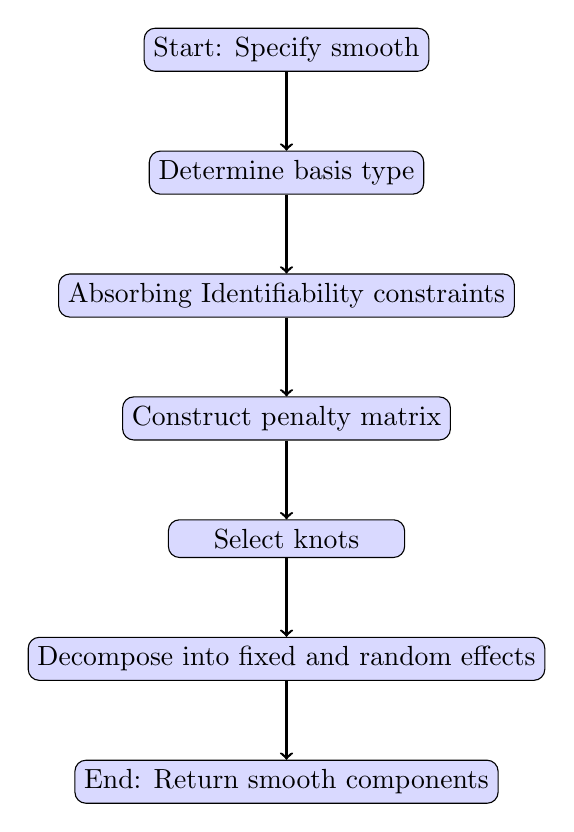
\begin{tikzpicture}[
    node distance=1cm,
    start chain=going below,
    every join/.style={->},
    every node/.style={draw, rounded corners, fill=blue!15, align=center, minimum width=3cm},
    arrow/.style={thick, ->}
]

% Nodes
\node (start) [on chain, join] {Start: Specify smooth};
\node (basis) [on chain, join] {Determine basis type};
\node (Absorb) [on chain, join] {Absorbing Identifiability constraints};
\node (penalty) [on chain, join] {Construct penalty matrix};
\node (knots) [on chain, join] {Select knots};
\node (decompose) [on chain, join] {Decompose into fixed and random effects};
\node (end) [on chain, join] {End: Return smooth components};

% Arrows
\draw [arrow] (start) -- (basis);
\draw [arrow] (basis) -- (Absorb);
\draw [arrow] (Absorb) -- (penalty);
\draw [arrow] (penalty) -- (knots);
\draw [arrow] (knots) -- (decompose);
\draw [arrow] (decompose) -- (end);

\end{tikzpicture}
\caption{Schematic overview of the \texttt{smoothCon} function from \texttt{mgcv}.}
\end{figure}


The \texttt{smoothCon} function in \texttt{mgcv} is a core utility designed to process smooth specifications in generalized additive models (GAMs). It essentially sets up the necessary matrices and information for representing and estimating the smooth components in the model. Here's an overview of its operation:

\begin{enumerate}[label=\arabic*., left=0pt]
    \item \textbf{Input Specification}: The function takes in a smooth specification, which consists of a combination of a predictor variable, a basis type (\texttt{bs} argument), and other options like the number of knots (\texttt{k} argument).
    
    \item \textbf{Determine Basis Type}: Based on the \texttt{bs} argument, \texttt{smoothCon} determines the type of basis functions to use. This choice influences the flexibility and shape of the smooth term. Common basis types include cubic splines (\texttt{cr}), thin plate splines (\texttt{tp}), and P-splines (\texttt{ps}), among others.

    \item \textbf{Absorbing Identifiability constraints}: \texttt{absorbs.cons=TRUE} ensures that the smooth terms are uniquely distinguishable and not confounded with other model components, like the intercept. The process employs QR decomposition, a mathematical method for transforming the basis functions such that they become orthogonal to the space of the constraints (e.g., the intercept). This orthogonality is essential because it prevents the overlap of effects between the smooth terms and the intercept, ensuring that each component of the model contributes distinctly to the explanation of the data. 

    
    \item \textbf{Construct Penalty Matrix}: One of the fundamental aspects of GAMs is the application of a penalty to the smooth terms to avoid overfitting. \texttt{smoothCon} constructs a penalty matrix appropriate for the chosen basis type. The penalty typically targets the "wiggly" parts of the smooth to ensure a balance between fit and smoothness.
    
    \item \textbf{Select Knots}: Knots are specific points in the data range where the spline functions can change direction. \texttt{smoothCon} selects appropriate knot locations based on the data and the specified number of knots (\texttt{k} argument).
    
    \item \textbf{Decompose into Fixed and Random Effects}: For certain applications, especially when using GAMs in mixed model frameworks, the smooth terms can be decomposed into fixed and random effects components. \texttt{smoothCon} provides the necessary decomposition, allowing the smooth to be used in packages like \texttt{gamm4}.
    
    \item \textbf{Output}: The function returns a list containing various components representing the smooth, including the basis functions, penalty matrices, and other relevant information.
\end{enumerate}


\subsection{Re-parametrizing Using smooth2random}

\begin{figure}[h]
\centering
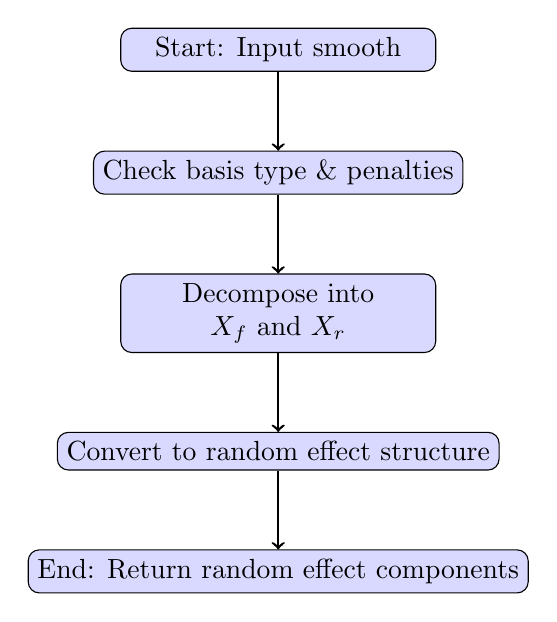
\begin{tikzpicture}[
    node distance=1cm, 
    start chain=going below,
    every join/.style={->},
    every node/.style={draw, rounded corners, fill=blue!15, align=center, minimum width=4cm},
    arrow/.style={thick, ->}
]

% Nodes
\node (start) [on chain] {Start: Input smooth};
\node (check) [on chain, join] {Check basis type \& penalties};
\node (decompose) [on chain, join] {Decompose into \\ \(X_f\) and \(X_r\)};
\node (convert) [on chain, join] {Convert to random effect structure};
\node (end) [on chain, join] {End: Return random effect components};

% Arrows
\draw [arrow] (start) -- (check);
\draw [arrow] (check) -- (decompose);
\draw [arrow] (decompose) -- (convert);
\draw [arrow] (convert) -- (end);

\end{tikzpicture}
\caption{Schematic overview of the \texttt{smooth2random} function from \texttt{mgcv}.}
\end{figure}

The \texttt{smooth2random} function in the \texttt{mgcv} package serves as a vital bridge between the realm of Generalized Additive Models (GAMs) and Generalized Linear Mixed Models (GLMMs). Its primary role is the transformation of smooth terms, typically utilized within GAMs, into a format that aligns with the structural requirements of random effects in GLMMs.

\begin{itemize}
    \item \textbf{Purpose}: The function's design facilitates the seamless integration of intricate spline-based effects into mixed models. This incorporation allows for the modeling of complex non-linear relationships, especially in scenarios with hierarchical or grouped data structures.
    
    \item \textbf{Functionality}: By converting smooth terms into random effect structures, \texttt{smooth2random} broadens the modeling capabilities, enabling researchers and analysts to capture and represent non-linear trends and patterns more effectively.
    
    \item \textbf{Impact}: The utility of \texttt{smooth2random} is especially pronounced in advanced modeling contexts, where the flexibility of GAMs is desired alongside the group-specific random effects of GLMMs.
\end{itemize}

In essence, \texttt{smooth2random} plays a pivotal role in expanding the horizons of mixed modeling, fusing the best of both GAMs and GLMMs to provide a robust toolset for statistical modeling.

\newpage




\subsection{How s() can be presented in \textbf{glmmTMB}}

While using the two functions we have mentioned above we can make the smoothing term in a \textbf{glmmTMB}-model.
\subsection*{R Code}

\begin{verbatim}
sm_tmpd <- mgcv::smoothCon(s(tmpd), absorb.cons = TRUE, 
                           data = chicago)[[1]]             
re_tmpd <- mgcv::smooth2random(sm_tmpd, "", type = 2)
Xf_tmpd <- re_tmpd$Xf
Xr_tmpd <- re_tmpd$rand[[1]]
chicago$ID <- factor(rep(1, nrow(chicago)))
ftmb1 <- glmmTMB(formula = death ~ Xf_tmpd +
                 homdiag(0 +Xr_tmpd | ID), 
                 data = chicago, REML=TRUE)
\end{verbatim}

\subsection*{Code Description}

\begin{enumerate}
    \item \textbf{Identifiability Constraints and Basis Function:}
    The code initializes a smooth term (\texttt{sm\_tmpd}) using \texttt{mgcv::smoothCon} with identifiability constraints absorbed into the basis, applicable to the variable \texttt{tmpd} in the \texttt{chicago} dataset.

    \item \textbf{Conversion to Random Effects:}
    The smooth term is then converted into random effects (\texttt{re\_tmpd}) using \texttt{mgcv::smooth2random}, specifying the type of conversion.

    \item \textbf{Extraction of Matrices:}
    Fixed effects matrix (\texttt{Xf\_tmpd}) and random effects matrix (\texttt{Xr\_tmpd}) are extracted from the converted smooth term.

    \item \textbf{Creating a Grouping Variable:}
    A fake grouping variable (\texttt{ID}) is created in the \texttt{chicago} dataset, assigning the same value to all observations for modeling purposes.

    \item \textbf{Generalized Linear Mixed Model (GLMM):}
    A GLMM (\texttt{ftmb1}) is fitted using \texttt{glmmTMB} to predict \texttt{death}, based on fixed effects and a random effect structure with a homogenous diagonal covariance structure, using Restricted Maximum Likelihood for estimation.
\end{enumerate}

\textbf{Note:} Type 1 Random Effects are akin to random intercepts in mixed models, where each group level has its own intercept, modeled using \texttt{s()} with \texttt{bs = "re"}. Type 2 Random Effects handle more complex variations like smooth random effects or random slopes, where each group level gets its own smooth function, implemented using \texttt{s()} with a grouping factor, as in \texttt{s(x, bs="fs", m=1, by=factor)}.


\subsection{Basis functions in \textbf{glmmTMB}}



\begin{table}[H]
\centering
\caption{Compatibility of Spline Types in \texttt{glmmTMB}}
\begin{tabular}{lccc}
\toprule
Spline & bs & Compatible & Reasoning \\
\midrule
Cubic Regression & \texttt{"cr"} & \checkmark &  \\
Cyclical Cubic & \texttt{"cc"} & $\times$ & Only one Xf-term \\
Cubic Smoothing & \texttt{"cs"} & $\times$ &  No Xf-terms \\
Thin Plate Regression & \texttt{"tp"} & \checkmark &   \\
B-splines & \texttt{"bs"} &  \checkmark &  \\
P-splines & \texttt{"ps"} &  \checkmark &  \\
Two-dimensional Tensor Product & \texttt{"t2"} & $\times$ & \\
Two-dimensional Tensor Product & \texttt{"te"} & $\times$ & Not supported by smooth2random (gamm4) \\
Shrinkage Smooth & \texttt{"fs"}  & \checkmark & \\
Adaptive & \texttt{"ad"}  &$\times$ & Not supported by smooth2random  \\
Random Effect & \texttt{"re"}  & $\times$ & No Xf-terms \\
% Add other splines as needed
\bottomrule
\end{tabular}
\end{table}


\subsubsection{Proposition for\texttt{ bs="cs"} and \texttt{bs="cc"}}

The cyclical cubic regression spline and cubic smoothing spline do not have these \texttt{Xf} terms, fixed effects, and the model will therefore not work with the code given is section 5.3. A seemingly nice alternative would be to code the model without the \texttt{Xf} terms, as all the information from these basis funtions are given in the \texttt{Xr} terms:

\begin{verbatim}
    ftmb1 <- glmmTMB(formula = death ~ 
    homdiag(0+Xr_tmpd | fake_group)
    , data = chicago, REML=TRUE)
\end{verbatim}

Later in the thesis we will do some comparison between this formula and a corresponding \textbf{GAM} model with basis functions of cyclical and cubic smoothing splines to prove that it may be a solution.



\subsection{Complexities of Tensor Product Splines}

Smooths of tensor product splines are more complicated and challenging to implement, due to their more complex construction and structure. One obstacle is handling the splitting of the model matrix into 4 matrices, three of which are \texttt{Xr}-matrices and one \texttt{Xf}-matrix. There is comprehensive mathematical theory on which construction methods for tensor product smooths are built (see \cite{wood2017}). Understanding the finer details and mechanisms of how tensor product splines are constructed by the smooth constructor is crucial for managing their implementation in glmmTMB. 

\subsubsection{Tensor Product Construction of Smooths in GAMs}

Fabian Scheipl's alternative tensor product construction in \texttt{mgcv} facilitates smooth term estimation using a method which simplifies mixed modeling by using non-overlapping penalty terms \cite{wood2017}. This construction yields a model with easily interpretable, rescaling-invariant smooth terms suitable for mixed effect modeling.

We begin with a set of unconstrained marginal smooths. The next step involves re-parameterizing each marginal so that the penalty matrix becomes an identity matrix, with \( M \) leading diagonal entries zeroed (\( M \) being the dimension of the penalty null space. This step includes a linear rescaling of parameters to equate the positive elements of the penalty matrix to 1.
\newline

We then divide each re-parameterized model matrix into columns \( \mathbf{X} \) and \( \mathbf{Z} \). \( \mathbf{X} \) corresponds to the zero elements on the leading diagonal of the penalty, and \( \mathbf{Z} \) to the unit entries, leading to \( \boldsymbol{f} = \mathbf{X} \boldsymbol{\delta} + \mathbf{Z}\boldsymbol{b} \). To enhance interpretability, it's preferable to have the constant function explicitly present in each marginal basis. An automatic re-parameterization method ensures this in the general case. For some function \( g \) in the penalty null space, the additional penalty \( P_N = \sum_i (g(x_i) - \bar{g})^2 \) shrinks \( g \) towards a constant function, i.e \( P_N = \boldsymbol{\delta}^T \mathbf{D}^T \mathbf{D} \boldsymbol{\delta} \), where \( \mathbf{D} = \mathbf{X}^{-1}_{1^T} \mathbf{X}/n \) and decomposed \( \mathbf{D}^T \mathbf{D} = \mathbf{U} \mathbf{\Omega} \mathbf{U}^T \).
\newline

Reparameterizing such that the null space model matrix is now \( XU \) ensures that the final column of the new model matrix is constant, assuming the original penalty's null space includes the constant function in its span.

For the \( d \) marginal smooths, the \( j \)th marginal has unpenalized model matrix \( X_j \) and penalized model matrix \( Z_j \) (with penalty \( I \)). We initialize matrices \( \gamma = \{X_1, Z_1\} \), or \( \gamma = \{[X_1], Z_1\} \) where \( [X_j] \) denotes the set of columns of \( X_j \), each treated as a separate matrix. The following steps are repeated for \( i \) from 2 to \( d \):

\begin{enumerate}
    \item Form row-wise Kronecker products of \( X_i \) (or of all columns \( [X_i] \)) with all elements of \( \gamma \).
    \item Form row-wise Kronecker products of \( Z_i \) with all elements of \( \gamma \).
    \item Append the matrices from the previous steps to the set \( \gamma \).
\end{enumerate}

The model matrix, \( X \), for the tensor product smooth is formed by appending all elements of \( \gamma \) columnwise. Each element of \( \gamma \) has an associated identity penalty with a smoothing parameter, except for elements involving no \( Z_j \) term, which are unpenalized. The variant using \( [X_j] \) instead of \( X_j \) ensures strict invariance with respect to linear rescaling of the covariates but requires extra penalty terms.

\begin{figure}[H]
    \centering
    \includegraphics[width=0.9\textwidth]{visuals/tensor_product_smooth.png}
    \caption{Tensor product smooth construction illustrated through a symmetric process in x and z dimensions. A smooth function \(f(z)\) is represented with a spline using six equidistant knots, with parameters varying smoothly along the \(x\)-axis. Each function parameter of \(f(z)\) is then modeled as a spline of \(x\). Scale invariance is ensured since separate smoothness penalties are applied in both the \(z\) and \(x\) directions. An \(x\)-direction penalty is formulated by summing \(\int \left[ f''(x) \right]^2 dx\) along the defined thin black curves. Similarly for a z-direction penalty.   \cite{wood2020inference}}
    \label{fig:tps}
\end{figure}

\newpage

\subsection{Modeling Convergence Issues with Smooths in \textbf{glmmTMB}}

Issues with convergence often arise due to insufficiently cleaned data, high model compolexity, or intricacies of the optimization algorithms used. Understanding these convergence problems is crucial for effective model fitting and accurate results.
\newline

Convergence issues can manifest in various forms, each with its unique characteristics and implications. For instance, problems with the Hessian matrix indicate issues with the solution's uniqueness, while difficulties in iteration or function optimization signal the need for algorithmic adjustments. Local minima, extreme eigenvalues, and false convergence are other examples of challenges that can complicate model fitting. A brief overview of optmizers and convergence problems are given in the tables below:

\subsubsection{Optimizers in \texttt{R} and \texttt{TMB}}

\begin{table}[ht]
\centering
\begin{tabular}{lll}
\toprule
\textbf{Optimizer} & \textbf{Environment} & \textbf{Primary Use Cases} \\
\midrule
Nelder-Mead & R & Unconstrained multi-dimensional optimization \\
BFGS & R & Nonlinear optimization problems \\
L-BFGS-B & R & Bounded optimization \\
CG & R & Large-scale optimization problems \\
SANN & R & Global optimization in complex landscapes \\
nlm & R & Unconstrained optimization using Newton-type method \\
nlminb & R & Bounded/unconstrained optimization \\
optimx & R & Unified interface for various methods \\
Newton & TMB & Maximum likelihood estimates \\
Limited-memory BFGS & TMB & Large models optimization \\
Conjugate Gradient & TMB & Large-scale problems in TMB \\
CppAD and Ipopt & TMB & Complex models with automatic differentiation \\
\bottomrule
\end{tabular}
\caption{Summary of Optimization Algorithms in R and TMB}
\label{tab:optimizers}
\end{table}



\begin{table}[H]
\centering
\begin{tabular}{>{\raggedright}p{4.5cm} >{\raggedright}p{6cm} >{\raggedright\arraybackslash}p{5.5cm}}
\toprule
\textbf{Model Convergence Issue} & \textbf{Description} & \textbf{Potential Solutions} \\
\midrule
Non-Positive-Definite Hessian Matrix & Occurs when the Hessian matrix at the solution is not positive definite, suggesting a non-unique solution or saddle point. & Check model specification, simplify the model, or provide better initial values. In cases where REML struggles to converge due to the model's complexity or data limitations, switching to ML might provide a more straightforward path to convergence. \\
\addlinespace
Iteration Limit or Objective Function Failure & Optimization algorithm didn't converge within iterations or failed to improve the objective function. & Increase iterations and evaluations, adjust CONVERGE value, or try different optimization methods. \\
\addlinespace
Inadequate Convergence or Local Minimum & Convergence criterion might only approximate a minimum point or converge to a local minimum. & Use different starting values, adjust convergence criteria, or employ a grid search for global minimum. \\
\addlinespace
Extreme Eigenvalues or False Convergence & Extreme eigenvalues suggest ill-conditioning, while false convergence indicates issues with gradient computati   on or tolerances. & Rescale data, check multicollinearity, restart the model with different starting values, or use alternative optimizers. \\
\addlinespace
Discontinuities or NA/NaN Evaluations & Discontinuities in the model or optimizer visiting invalid parameter spaces. & Ensure parameter estimates lie in a continuous interval, avoid discontinuity points, and ensure the optimizer leaves invalid regions. \\
\bottomrule
\end{tabular}
\caption{Common Convergence and Model-Fitting Issues in R for Non-Linear Models and GAMs}
\label{tab:model_convergence_combined}
\end{table}

\newpage

\section{Comparing Penalized vs Unpenalized Models}

In this section we'll demonstrate how penalization (and regularization generally) impacts accuracy and overfitting in spline regression models. 

\subsection{Implicit Regularization and Explicit Penalization}

In spline regression, model complexity control and overfitting prevention are typically addressed through two primary approaches: \textit{implicit/local control regularization} and \textit{explicit penalization}. The following table outlines the key characteristics of these approaches:

\begin{table}[H]
\centering
\begin{tabular}{|p{0.45\linewidth}|p{0.45\linewidth}|}
\hline
\textbf{Implicit/Local Control Regularization} & \textbf{Explicit Penalization} \\ \hline
\textbf{Number of Knots:} The number of knots controls the spline's flexibility. An appropriate number of knots allow for balancing flexibility and overfitting. & \textbf{Penalization of Wiggliness/Curvature:} A penalty on the curvature (second derivative) of the spline, such as the Integrated Squared Second Derivative (ISSD), ensures a smoother curve by discouraging excessive bending. \\ \hline
\textbf{Location of Knots:} Strategic placement of knots in areas with more data variation can improve the model's fit without increasing its complexity unnecessarily. & \textbf{Penalization of Coefficient Size (Ridge Penalty):} A quadratic penalty (akin to Ridge regression) on the spline coefficients prevents overfitting by constraining their magnitude, leading to a more robust model. \\ \hline
\textbf{Basis Functions:} An toptimal choice of basis functions, like TPRS or cubic smoothing splines, (which have different degrees of inherit wigglyness / smoothness), can strike a balance between flexibility and smoothness. &  \textbf{Penalization of Variance (PCR):} Indirectly penalize variance (complexity) by focusing on the principal coponents that explain the most of the variance in the predictors. \\ \hline
\end{tabular}
\caption{Comparison of Implicit/Local Control Regularization and Explicit Penalization in Spline Regression}
\label{tab:regularization_penalization}
\end{table}

In spline regression, the concurrent use of implicit/local control regularization and explicit penalization offers a compounded approach to model regularization. This dual strategy enhances the model's ability to balance complexity and overfitting. Implicit regularization, achieved through selecting knots and basis functions, establishes the foundational structure of the model, moderating its flexibility. Explicit penalization then complements this by targeting residual issues of excessive curvature or unduly large coefficients that may persist even after implicit regularization. By integrating these methods, we effectively compound their effects, ensuring a more nuanced control over the model. This synergy not only captures the data's underlying trends more accurately but also enhances the model's robustness and generalizability, particularly in complex statistical scenarios.

\subsection{Comparing Implicitly vs Explicitly Penalized Models}

Here we'll compare four different models. 

\begin{verbatim}
    tmb1 <- death ~ s(tmpd, k = 50), data = train_data)
    tmb2 <- death ~ homdiag(Xr_tmpd_tmb2|ID), data = train_data)
    tmb3 <- death ~ 1 + Xr_tmpd_tmb3, data = train_data)
    tmb4 <- death ~ 1 + Xr_tmpd_tmb4, data = train_data)
\end{verbatim}

\begin{itemize}
    \setlength{\itemsep}{1em} % Adjust the space between items
    \item \texttt{tmb1}: Bolker's implementation of smooths in glmmTMB. Sophisticated method, which in essence hacks \texttt{homdiag()} to the \texttt{s()} function of \texttt{mgcv}.
    \item \texttt{tmb2}: Johnson method using the \texttt{s2rPred} function and a manually specified \texttt{map} argument. The smooth has \texttt{k = 50, bs="tp"}.
    \item \texttt{tmb3}: Simply fitting the random basis function matrix of the smooth term as a fixed effect (k = 50, bs = "tp").
    \item \texttt{tmb4}: Same as above, but with more carefully chosen knot and basis function selection choices. The smooth has \texttt{k = 5, bs="cs"}.  
\end{itemize}


\begin{figure}[H]
    \centering
    \includegraphics[width=0.9\textwidth]{visuals/overfit_tmb1234_pred_vs_act.png}
    \caption{predicted vs actuals values on unseen test data of \texttt{tmb1, tmb2, tmb3 and tmb4}. Clearly \texttt{tmb3} (which is unpenalized) is not performing well on the test data, indicating that it overfits the data severely. }
    \label{fig:predicted_vs_actual_reglines_tmb1234}
\end{figure}




\section{Researching Improvements for \textbf{s()} in \textbf{glmmTMB}}



\subsection{Optimizing basis functions}

In section 5.4.1 we presented a possible option for cubic smoothing splines and cyclical cubic regression splines. 
This approach utilized a model only using the \texttt{Xr} terms, as all the information outputted from the \texttt{smooth2random} function is implemented in these terms.
\newline

Using the same tests as Bolker has used in his smooths.rmd file, we can see if this approach is similar to the way the \textbf{mgcv}-package handles the same type of smoothing. We will use the same data set as before, \texttt{chicago} from the R-package \textbf{gamair}.


\subsubsection{Presentation of models}

We introduce three distinct models developed using the \texttt{glmmTMB} function. Each model employs different smoothing techniques and structural compositions, tailored to the analysis of mortality data in the Chicago dataset. The models are delineated as follows:

\begin{itemize}
    \item \textbf{Model 1 (ftmb1)}: This model incorporates both fixed and random effects. The formula used is: 
    \begin{verbatim}
    ftmb1 <- glmmTMB(formula = death ~ Xf_tmpd +
             homdiag(0 + Xr_tmpd | fake_group), data = chicago,
             REML = TRUE)
    \end{verbatim}
    It combines a linear term for temperature (\texttt{Xf\_tmpd}) with a random smooth term (\texttt{Xr\_tmpd}) grouped by \texttt{fake\_group}, the same way a smoothing function on the temperature would do.

    \item \textbf{Model 2 (ftmb1cs)}: This model focuses solely on the random smooth term using cubic splines (CS) for smoothing as all the information is merged in the random component:
    \begin{verbatim}
    ftmb1cs <- glmmTMB(formula = death ~ 
    homdiag(0 + Xr_tmpdcs | fake_group), 
               data = chicago, REML = TRUE)
    \end{verbatim}
    Here, \texttt{Xr\_tmpdcs} represents the cubic spline transformation of the temperature data.

    \item \textbf{Model 3 (ftmb1cc)}: Similar to Model 2, this model uses cyclic cubic splines (CC) for the random smooth term:
    \begin{verbatim}
    ftmb1cc <- glmmTMB(formula = death ~ 
    homdiag(0 + Xr_tmpdcc | fake_group),
               data = chicago, REML = TRUE)
    \end{verbatim}
    The term \texttt{Xr\_tmpdcc} denotes the cyclic cubic spline transformation applied to the temperature data.
\end{itemize}



Each model serves a unique purpose in the analysis, offering insights into the effects of temperature on mortality rates under different smoothing assumptions.



\subsubsection{Comparison}

The effectiveness of various smoothing techniques in generalized additive models, specifically TPRS, CS, and CC smoothing, can be evaluated by comparing their mean relative differences in residual standard error and fitted values, as Bolker also demonstrated in his rmd.file. The analysis focuses on two aspects: the mean relative differences for various smoothing types (Table \ref{tab:smoothing_differences}) and the mean relative differences for fitted values in smoothing techniques (Table \ref{tab:fitted_values_smoothing_differences_sci})

\subsubsection*{Residual Standard Error}

\begin{table}[h]
\centering
\begin{tabular}{|c|c|}
\hline
\textbf{Smoothing Type} & \textbf{Mean Relative Difference} \\ \hline
TPRS Smoothing         & \(4.192224 \times 10^{-5}\)        \\ \hline
CS Smoothing           & \(9.436679 \times 10^{-5}\)        \\ \hline
CC Smoothing           & \(1.718639 \times 10^{-4}\)                   \\ \hline
\end{tabular}
\caption{Mean Relative Differences for Various Smoothing Types}
\label{tab:smoothing_differences}
\end{table}





\subsubsection*{Fitted Values}

\begin{table}[h]
\centering
\begin{tabular}{|c|c|}
\hline
\textbf{Smoothing Type} & \textbf{Mean Relative Difference} \\ \hline
TPRS Smoothing         & \(3.131819 \times 10^{-4}\)        \\ \hline
CS Smoothing           & \(5.668919 \times 10^{-4}\)        \\ \hline
CC Smoothing           & \(1.018736 \times 10^{-3}\)        \\ \hline
\end{tabular}
\caption{Mean Relative Differences for Fitted Values in Smoothing Techniques}
\label{tab:fitted_values_smoothing_differences_sci}
\end{table}




The effectiveness of various smoothing techniques in generalized additive models, specifically TPRS, CS, and CC smoothing, can be evaluated by comparing their mean relative differences in residual standard error and fitted values. The analysis focuses on two aspects: the mean relative differences for various smoothing types (Table \ref{tab:smoothing_differences}) and the mean relative differences for fitted values in smoothing techniques (Table \ref{tab:fitted_values_smoothing_differences_sci}).



Based on these observations, it can be inferred that while CS and CC smoothing are effective, TPRS smoothing demonstrates a marginally superior performance in terms of mean relative differences in both residual standard error and fitted values. However, the differences are relatively small, suggesting that CS and CC smoothing can be considered as viable alternatives to TPRS, especially in scenarios where specific model characteristics or data types may favor these methods.

\textit{Note:} The effectiveness of a smoothing technique can also be context-specific and depend on various factors such as the nature of the data, the complexity of the model, and the specific requirements of the analysis.


\subsubsection*{AIC and LogLik}

\begin{table}[h]
\centering
\begin{tabular}{|l|c|c|c|c|}
\hline
\textbf{Model Type} & \textbf{MGCV logLik} & \textbf{TMB logLik} & \textbf{MGCV AIC} & \textbf{TMB AIC} \\ \hline
TPRS               & -20718.41            & -20735.68           & 41456.82          & 41479.36         \\ \hline
CS                 & -20716.70            & -20738.91           & 41454.01          & 41483.81         \\ \hline
CC                 & -20718.82            & -20739.39           & 41457.23          & 41484.78         \\ \hline
\end{tabular}
\caption{Comparison of AIC and logLik Values for MGCV and TMB Models}
\label{tab:mgcv_tmb_comparison}
\end{table}


\subsection{Removing Model Convergence Issues }


\subsubsection{Non-positive-definite Hessian Matrix}

 To replicate the output Bolker get we have to use REML in our models, as he has described in his R-markdown file \texttt{smooths}. It is stated that this should be done to avoid convergence failure, however, when we have done our research we have encountered a lot of convergence issues using REML, especially of the form non-positive-definite hessian matrix. 
 \newline
 When changing the models to only using ML fit, this problem went away, and we developed some good models. 
 \newline
 On the other hand, we also encountered some opposite examples, where the ML fit gave convergence failure, but REML worked fine.

\section{Domains for Spline Regression Application}

While spline regression models find applicability across a diverse array of phenomena, ranging from biological sciences to engineering, our focus on financial time series, insurance data, and large weather data is rooted in their particular relevance to the field of actuarial science. This selection aligns closely with the core areas of actuarial expertise, which include financial modeling, risk assessment, and quantitative analysis. Financial time series data is pivotal in understanding market dynamics and risk, essential for financial planning and investment strategies. Insurance data is at the heart of actuarial science, where accurate risk modeling is key to premium setting and risk management. Lastly, large weather data is increasingly crucial in actuarial work, especially considering the growing impact of climate change on risk calculations and insurance models. These domains not only provide a rich context for applying spline regression models but also are highly pertinent to the evolving role of actuaries in a world where data-driven decision-making is paramount.


\subsection{Financial Time Series Data}
In the realm of financial markets, characterized by inherent volatility and complex, non-linear dynamics, spline regression emerges as a particularly potent tool. It adeptly captures the intricate patterns observed in stock prices, interest rates, and market indices, accommodating for the frequent shifts and trends triggered by economic events, policy changes, and market sentiments. The flexibility of spline models in adapting to these abrupt fluctuations makes them invaluable for forecasting market movements, optimizing risk management, and identifying lucrative trading opportunities.

\subsubsection{Time Series Analysis}

We'll start off with some theory on time series analysis. In financial contexts it involves several critical considerations to accurately capture and predict complex temporal dynamics. Key concepts and methodologies are outlined below to guide this analytical process.
\newline

\subsubsection*{Definition of Auto-Correlation}

Auto-correlation, also known as serial correlation, refers to the correlation of a time series with its own past and future values. Mathematically, the auto-correlation function \(ACF\) for a time series \( \{X_t\} \) is defined as:

\[
ACF(\tau) = \frac{\text{Cov}(X_t, X_{t-\tau})}{\sqrt{\text{Var}(X_t) \times \text{Var}(X_{t-\tau})}}
\]

where \( \tau \) is the time lag, and \( \text{Cov} \) and \( \text{Var} \) are the covariance and variance, respectively.

\subsubsection*{Prevalence in Financial Time Series Data}

Auto-correlation is particularly prevalent in financial time series data for several reasons:

\begin{itemize}
    \item \textbf{Market Trends}: Financial markets often exhibit trends that persist over time, leading to positive auto-correlation.
    \item \textbf{Seasonality}: Many financial instruments show seasonal patterns, such as increased retail stock prices before holidays, which introduce auto-correlation.
    \item \textbf{Liquidity Constraints}: Trading restrictions or liquidity constraints can delay trading actions, causing a lagged effect and thus auto-correlation.
    \item \textbf{Information Diffusion}: Information takes time to propagate among market participants, leading to a gradual adjustment of prices and hence auto-correlation.
\end{itemize}

\subsubsection*{Implications}

The presence of auto-correlation in financial time series data has important implications:

\begin{itemize}
    \item \textbf{Modeling}: Traditional models like ordinary least squares (OLS) regression assume no auto-correlation; thus, specialized models like ARIMA or GARCH may be more appropriate.
    \item \textbf{Risk Assessment}: Auto-correlation can affect the volatility and predictability of financial instruments, impacting risk assessments.
    \item \textbf{Trading Strategies}: Understanding auto-correlation can help in developing more effective trading strategies, such as momentum or mean-reversion strategies.
\end{itemize}

\subsubsection*{Detection and Treatment}

Auto-correlation is commonly detected using statistical tests like the Durbin-Watson test or by examining the ACF and Partial Auto-Correlation Function (PACF) plots. Once detected, it can be treated or modeled using techniques like differencing, or by using models that explicitly account for auto-correlation, such as ARIMA or GARCH models.


\begin{itemize}
  \item Differencing: Transforming the series to a stationary one by differencing data points with their previous values.
  \item ARIMA models: Integrating autoregressive (AR) and moving average (MA) components to model the time series effectively.
  \item Lagged variables: Including past values as predictors in the regression model.
\end{itemize}


\subsubsection*{Overview of ARIMA Models}

ARIMA, standing for AutoRegressive Integrated Moving Average, is a class of models that capture various standard temporal structures in time series data. The model is typically denoted as \(ARIMA(p, d, q)\), where \(p\) is the order of the AutoRegressive (AR) term, \(d\) is the number of differencing required to make the time series stationary, and \(q\) is the order of the Moving Average (MA) term.

Mathematically, an ARIMA model is expressed as:

\begin{equation}
    \phi(B)(1-B)^d X_t = \theta(B)Z_t,
    \label{eq:arima}
\end{equation}

where \( \phi(B) \) and \( \theta(B) \) are the AR and MA polynomials in the backshift operator \( B \), \( X_t \) is the time series, and \( Z_t \) is white noise. ARIMA models are effective for modeling a wide range of time series behaviors, including trends and auto-correlation, and are particularly useful for forecasting and anomaly detection, for example in financial data.

\subsubsection*{Seasonal ARIMA (SARIMA) Models}

SARIMA, or Seasonal ARIMA, extends the ARIMA model by explicitly accounting for seasonality in time series data. SARIMA models are denoted as \(ARIMA(p,d,q)(P,D,Q)_s\), where \(P\), \(D\), and \(Q\) are the seasonal orders of the AR, differencing, and MA components, respectively, and \(s\) represents the length of the seasonal cycle.

In SARIMA, the seasonal differencing involves subtracting the value from a previous season, thereby stabilizing the mean of a seasonal time series. These models are particularly suitable for datasets with clear seasonal patterns, such as monthly sales data or yearly temperature variations.

\subsubsection*{ARIMA with Exogenous Variables (ARIMAX)}

ARIMAX, or ARIMA with eXogenous variables, is an extension of the ARIMA model that incorporates external or independent variables. This is useful when the time series is thought to be influenced by factors outside of its own past values. 
\newline

The ARIMAX model is particularly valuable in scenarios where external events or interventions are known to impact the time series. For instance, in financial time series, external factors like changes in economic policy, market trends, or geopolitical events can be included to enhance the model's predictive accuracy.
\newline

By integrating these external variables, ARIMAX provides a more comprehensive modeling approach, improving forecasts and insights, especially in complex environments where multiple factors influence the time series.



\subsubsection*{Preserving the Temporal Structure During Analysis}
The integrity of time series data is intrinsically tied to its temporal structure, which records the sequential interdependence of observations. Maintaining this order is pivotal when modeling financial time series, where patterns and trends across time are of primary interest. We will deploy several appropriate techniques to ensure the temporal structure is maintained.


\subsection{Modelling Log-Returns Post-COVID-19 and the Rise of Meme Stocks}

The onset of the COVID-19 pandemic introduced a period of very high volatility in global financial markets. Traditional linear models faced challenges in capturing these complex dynamics, particularly in the years 2020 and 2021. This period was also marked by the emergence of "meme stocks," such as GameStop and AMC Entertainment Holdings. These stocks experienced dramatic increases in value, driven by retail investors influenced by social media and trading platforms like Robinhood and Webull \cite{reuters2021meme}. However, the trend was characterized by extreme fluctuations, with some stocks trading significantly below their peak values \cite{reuters2021meme2}. The increased use of options trading further exacerbated market swings \cite{reuters2021options}.
\newline
    
Spline regression, known for its flexibility in accommodating abrupt changes and non-linear trends, may emerge as a more suitable analytical tool in this context. It can offer deeper insights into the post-COVID-19 financial landscape and aided in the development of robust forecasting and risk management strategies during these turbulent times.
\newline

\begin{center}
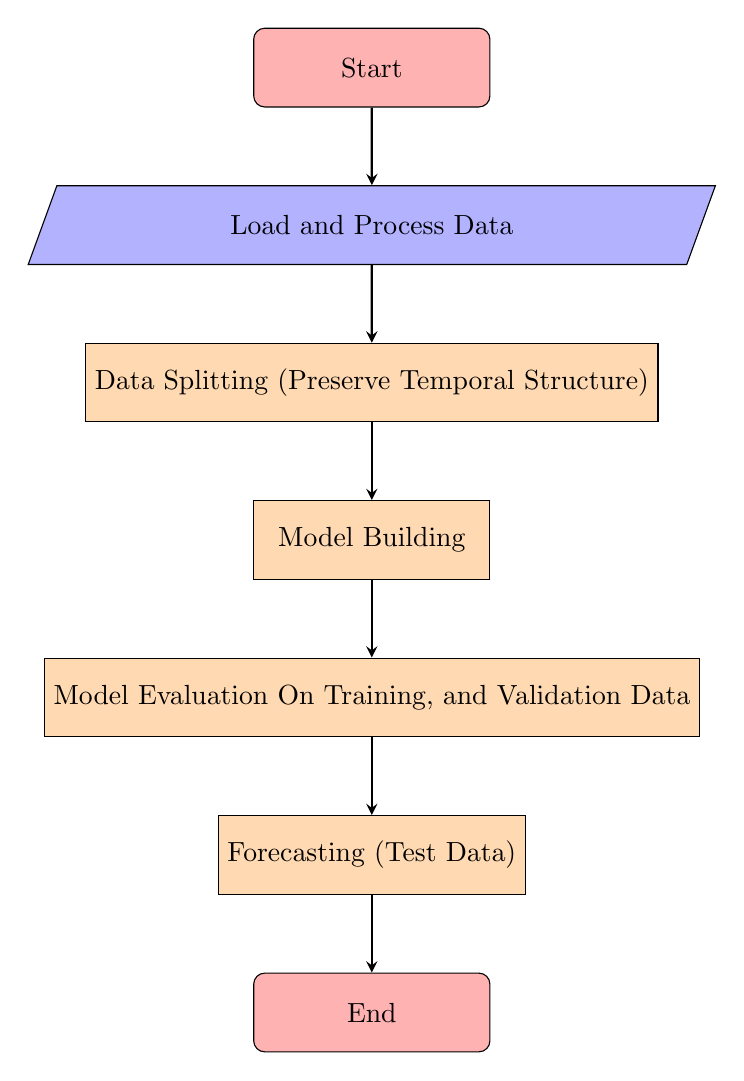
\begin{tikzpicture}[node distance=2cm]
\node (start) [startstop] {Start};
\node (data) [io, below of=start] {Load and Process Data};
\node (split) [process, below of=data] {Data Splitting (Preserve Temporal Structure)};
\node (model) [process, below of=split] {Model Building};
\node (evaluate) [process, below of=model] {Model Evaluation On Training, and Validation Data};
\node (forecast) [process, below of=evaluate] {Forecasting (Test Data)};
\node (end) [startstop, below of=forecast] {End};

\draw [arrow] (start) -- (data);
\draw [arrow] (data) -- (split);
\draw [arrow] (split) -- (model);
\draw [arrow] (model) -- (evaluate);
\draw [arrow] (evaluate) -- (forecast);
\draw [arrow] (forecast) -- (end);
\end{tikzpicture}
\end{center}

This figure illustrates the sequential steps involved in our time series regression analysis, highlighting the importance of data order preservation, model building with autocorrelation handling and non-linear modeling techniques, and thorough model evaluation before proceeding to forecasting.



\subsubsection{Analysis of the Model}

In this analysis, we focus on fitting three distinct models, but of the same form, using the \texttt{glmmTMB} package, each employing a different technique to approach spline regression. For the specific example demonstrated here, models of the form \texttt{log\_return $\sim$ s(time) + s(volume) + arima\_residuals, family = gaussian} were fitted, where the smooth terms in all models \textbf{TPRS} with \textbf{k = 10}. Bolker's method is more restricted in it's ability use other spline types (varying the bs=$"\cdot"$ parameter) than the other models, which are only constrained by the compatibility with \textbf{smooth2random}. The primary objective is to investigate key aspects such as efficiency, accuracy, and generalizability across these models.
\newline

The first model, referred to as \texttt{tmb1}, is a spline regression model that exclusively fits the "random part" — specifically, the matrix of basis functions denoted as \texttt{Xr}. In this model, these basis functions are estimated as fixed effects, with a manually implemented ridge penalty applied to regularize the model. This approach is expected to balance the model's flexibility with its ability to prevent overfitting, while being computationally efficient.
\newline

The second model, \texttt{tmb2}, mirrors \texttt{tmb1} in its form and structure. However, it distinctly lacks explicit regularization, meaning it does not include a ridge penalty. The comparison between \texttt{tmb1} and \texttt{tmb2} will provide insights into the impact of regularization on model performance, particularly in terms of accuracy and the risk of overfitting.
\newline

Finally, \texttt{tmb3} adopts the spline regression using Ben Bolker's version of a Generalized Additive Model (GAM) within \texttt{glmmTMB}. This model's implementation provides a more involved and sophisticated approach to spline fitting, but at the cost of computational efficiency. It will be serve as a comparison/benchmark. 


\subsubsection*{Data Preparation and Exploration}
Our program begins with data loading and preprocessing. Financial time series data, inherently non-linear and volatile, is loaded and prepared for analysis. This phase includes generating smooth terms and calculating ARIMA residuals, to enable effective spline modeling. 
\newline

\subsubsection*{Data Splitting Techniques}
We have meticulously ensured that the chronological sequence remains unaltered during data splitting for training, validation, and testing phases. Zero random sampling has been used in splitting data, only sequential cuts. We employed techniques such as rolling windows for cross-validation to preserve the contiguous nature of the data, thereby avoiding lookahead bias which can occur if future information is inadvertently incorporated into the model training process. Additionally, the residuals from the ARIMA models were used to account for autocorrelation within the time series, ensuring that the models capture the dependencies inherent in the data without being misled by spurious correlations. These measures collectively help safeguard the temporal structure, thus ensuring the reliability and validity of our model's predictions.

\subsubsection*{Ridge Penalty and Model Configuration}
A pivotal aspect of the program is the application of a ridge penalty in the spline regression model of interest. This regularization technique is crucial for managing the complexity of the models, avoiding overfitting, and enhancing predictive accuracy. Cross-validation is employed to determine the optimal lambda, the regularization parameter, ensuring the models strike a balance between flexibility and generalizability. Manually implementing the ridge penalty requires careful data augmentation which is described within the R-script. 

\subsubsection*{Model Fitting and Evaluation}
Three spline regression models are fitted on the prepared data — tmb1 with a ridge penalty, tmb2 as an unpenalized counterpart, and tmb3, a more sophisticated variant. Each model undergoes rigorous evaluation, including in-sample and cross-validation RMSE calculations, to assess predictive performance.
\newline

The three models will be assessed based on their computational efficiency (time taken for model fitting), accuracy (how closely the models predict the observed data), and generalizability (ability to perform well on unseen data, thus indicating resistance to overfitting). Through this comparative analysis, we aim to delineate the strengths and limitations of each modeling approach within the context of spline regression in financial time series data.


\subsubsection*{Advanced Model Analysis}
Beyond basic evaluations, the program delves into deeper analysis and diagnostics. This includes residual analysis, learning curve evaluation, and various statistical tests to comprehensively understand model behavior and effectiveness.


\subsubsection*{Visualization and Interpretation}
For complex models visualization is a vital tool for interpreting model results. Plots and graphical representations are generated for RMSE trends, residuals, learning curves, and predicted versus actual values, facilitating an intuitive understanding of model performance.

\subsection{Comparing and Interpreting the Results}


\subsubsection*{In-Sample and Training}


\begin{table}[h]
\centering
\begin{tabular}{|l|c|c|c|c|}
\hline
Model & In-Sample RMSE & Time (sec) & AIC & BIC \\
\hline
tmb1 & 0.03034 & 0.4472 & -2689.85 & -2604.56 \\
tmb2 & 0.03100 & 0.4283 & -2675.70 & -2590.63 \\
tmb3 & 0.03033 & 1.2957 & -2655.41 & -2624.08 \\
\hline
\end{tabular}
\caption{In-sample RMSE, Model Fitting Time, AIC, and BIC on Training Data}
\end{table}


\subsubsection*{Test Data}
\newpage

\begin{figure}[H]
    \centering
    \begin{subfigure}[b]{0.45\textwidth}
        \includegraphics[width=\textwidth]{visuals/Visuals_ts_ridge/hist_pred_errors.png}
        \caption{Histogram of Prediction Errors}
        \label{fig:hist_pred_errors}
    \end{subfigure}
    \hfill
    \begin{subfigure}[b]{0.45\textwidth}
        \includegraphics[width=\textwidth]{visuals/Visuals_ts_ridge/Predicted_vs_actual_densities_ts_ridge.png}
        \caption{Predicted vs Actual Densities}
        \label{fig:predicted_vs_actual_densities}
    \end{subfigure}
    \caption{Test Data Performance: Error Distribution and Density Comparison}
    \label{fig:test_data_performance_1}
\end{figure}


\begin{figure}[H]
    \centering
    \includegraphics[width=0.9\textwidth]{visuals/Visuals_ts_ridge/predicted_vs_actual_test_data_lines.png}
    \caption{Predicted vs Actual Values with Loess Regression}
    \label{fig:predicted_vs_actual_lines}
\end{figure}


\begin{table}[h]
\centering
\begin{tabular}{|l|c|}
\hline
Model & RMSE on Test Data \\
\hline
tmb1 & 0.03912 \\
tmb2 & 0.17445 \\
tmb3 & 0.09075 \\
\hline
\end{tabular}
\caption{RMSE for Models on Test Data}
\end{table}


\subsection{Model Performance Summary}

\subsubsection*{Efficiency Analysis}
The computational efficiency of the models revealed a notable difference in time complexity. Models \texttt{tmb1} and \texttt{tmb2} exhibited similar computation times, approximately 3.79 and 3.66 seconds, respectively. Model \texttt{tmb3} required more substantial computational resources, with a total computation time of around 9.60 seconds, indicating the computational cost of the Generalized Additive Model (GAM) approach within \texttt{glmmTMB}.

\subsubsection*{In-Sample Performance}
The in-sample Root Mean Squared Error (RMSE) comparison showed that \texttt{tmb1} and \texttt{tmb3} performed similarly, whereas \texttt{tmb2} reported a marginally higher RMSE. This suggests that \texttt{tmb2} may not capture the training data's underlying patterns as effectively due to the absence of regularization.

\subsubsection*{Validation and Learning Curve Analysis}
Throughout the learning curve analysis, \texttt{tmb1} consistently outperformed the other models in terms of RMSE on the validation data, indicating a superior ability to generalize. Conversely, \texttt{tmb2} displayed highly variable RMSE values, particularly with smaller training sets, hinting at a propensity for overfitting. \texttt{tmb3} showed moderate RMSE values, suggesting better generalizability than \texttt{tmb2} but less so compared to \texttt{tmb1}.

\subsubsection*{Cross-Validation Metrics}
Across the cross-validation folds, \texttt{tmb1} achieved the best average metrics, including RMSE, Mean Absolute Error (MAE), and Mean Absolute Percentage Error (MAPE), corroborating its predictive accuracy. \texttt{tmb2} had the least favorable results, further suggesting overfitting. \texttt{tmb3} performed better than \texttt{tmb2} and exhibited the highest average R-squared, indicating a strong fit to the data's variance.

\subsubsection*{Test Data Evaluation}
On the unseen test data, \texttt{tmb1} maintained the lowest RMSE, reinforcing its robustness. \texttt{tmb2}'s performance on the test data was subpar, with a significantly higher RMSE, while \texttt{tmb3} provided a reasonable fit but was not as precise as \texttt{tmb1}.

\subsubsection*{Information Criteria Comparison}
The Akaike Information Criterion (AIC) and Bayesian Information Criterion (BIC) favored \texttt{tmb1}, with the lowest values indicating the best model considering both fit and complexity. \texttt{tmb3} did not offer a better fit to justify its computational cost, and \texttt{tmb2} was less efficient than \texttt{tmb1} when complexity was accounted for.


\subsubsection*{Conclusion}

In conclusion, \texttt{tmb1} surfaces as the most advantageous model for this particular dataset, striking an optimal balance between efficiency, accuracy, and generalization capabilities. The selection of the appropriate model may depend on the specific requirements of the analysis, and the specific financial time series dataset; however, \texttt{tmb1} would likely be a good choice in many scenarios. The key difference between \texttt{tmb1} and \texttt{tmb3} is the penalty term, Ridge and ISSD respectively. The difference in performance is an interesting observation which warrants further investigation.




\subsection{Big Data}

The advent of "Big Data" has revolutionized the landscape of computational analysis and decision-making. Big Data refers to datasets that are so large or complex that traditional data processing applications are inadequate. The utility of Big Data lies in its ability to provide unprecedented insights and predictive power across various fields, from healthcare to finance. With the advancement of technologies such as machine learning and data mining, Big Data has become a cornerstone in driving innovations and efficiencies.
\newline

However, the complexity and challenges associated with Big Data cannot be understated. One of the primary concerns is the scalability of computational models as data size increases. The relationship between dataset size and computational complexity is often non-linear. As detailed in the research by Leskovec, Rajaraman, and Ullman (2014), the complexity of algorithms can scale superlinearly with data size, leading to exponentially increasing computational resource requirements and processing time.
\newline

Furthermore, the management and analysis of Big Data require significant computational resources, both in terms of hardware and software. As the size of the data grows, the time required for processing and analysis grows as well, often requiring parallel and distributed computing techniques to manage effectively. Empirical studies, such as those conducted by Dean and Ghemawat (2008) in the context of Google's MapReduce, demonstrate how distributed computing frameworks can manage and process large datasets, but also highlight the complexity and resource demands of such operations.
\newline

Another challenge in Big Data is ensuring data quality and integrity. The volume and variety of data often lead to inconsistencies, noise, and missing values, which can significantly affect the outcomes of data analysis. Addressing these issues requires additional preprocessing steps, further adding to the computational load.
\newline


\subsubsection{Challenges and Strategies in Modeling Large Datasets on Personal Computers}

Modeling large datasets on personal computers presents unique challenges due to the limitations of hardware resources and processing power. Unlike enterprise-level computational resources, personal computers have finite, often limited, capacities in terms of memory, storage, and processing capabilities. The complexity of computational models and the size of datasets typically scale non-linearly, which can have significant implications on hardware requirements and time usage.

\textbf{Non-Linear Scaling of Complexity}: Theoretical and empirical studies have shown that the computational complexity of algorithms used in data modeling often scales superlinearly with the size of the data. For instance, certain machine learning algorithms have a complexity of \( O(n^2) \) or even \( O(n^3) \), where \( n \) is the number of data points (Cormen et al., 2009). This non-linear scaling means that doubling the dataset size more than doubles the computational effort, leading to exponential increases in processing time and memory usage.

\textbf{Hardware Limitations}: On a typical modern personal computer, which may have between 4 to 16 cores, and in some state-of-the-art high-end models up to 96 cores, the challenge lies in efficiently utilizing these cores for parallel computation. The memory (RAM) is also a bottleneck; larger datasets require more memory, and once the available RAM is exceeded, the computer resorts to using slower disk-based storage, further impacting performance. A typical modern PC has 8-32GB of RAM, with very high end models having 64-128GB. 

\textbf{Strategies for Effective Modeling}:
\begin{itemize}
     \item \textit{Data Preprocessing}: Techniques such as dimensionality reduction, sampling, and data cleaning can significantly reduce the size of the dataset without substantial loss of information, making it more manageable for personal computers.
    \item \textit{Algorithm Optimization}: Choosing algorithms with lower complexity or optimizing existing algorithms to be more efficient can mitigate the effects of non-linear scaling. For example, using approximation algorithms or algorithms with linear time complexity can be more suitable for large datasets.
    \item \textit{Parallelization}: Utilizing the multi-core architecture of modern CPUs through parallelization can significantly reduce computation time. Techniques like multithreading or using parallel processing libraries allow for distributing the workload across multiple cores.
\end{itemize}

In conclusion, while modeling large datasets on personal computers is challenging due to hardware limitations and the non-linear scaling of model complexity, strategies like data preprocessing, algorithm optimization, and parallelization provide viable pathways to effectively manage and analyze large datasets.

\subsubsection{Parallelization and Optimization}

Parallelization in statistical models and computing represents a pivotal shift in the way data analysis is performed in a multi-core and distributed computing environment. Traditionally, computational tasks in statistics are performed sequentially, but parallelization breaks these tasks into smaller, independent sub-components that can be executed concurrently. This approach is particularly transformative in statistical modeling, where processes such as simulations, bootstrapping, or cross-validation are inherently repetitive and can be parallelized effectively.
\newline

The benefit of parallelization is most pronounced in the context of handling complex models and large datasets. For example, complex climate and weather models that use long running historical data, to model and predict non-linear relationships between continous variables. 
\newline

The rise of parallel computing has spurred the development of new statistical methodologies and software designed for parallel execution. This includes the integration of parallel processing capabilities in popular programming languages like R and Python, offering statisticians and data scientists the tools to implement parallelization with ease. However, parallelization also introduces challenges such as synchronization, managing data dependencies, and the overhead associated with task distribution and result integration. Nonetheless, the advantages of parallelization, especially in handling extensive data analyses and complex statistical models, are substantial, underscoring its essential role in contemporary statistical computing.

\subsubsection*{Parallelization in R using \texttt{furrr} and \texttt{future} Packages}

The implementation of parallelization in R has been greatly enhanced with the introduction of the \texttt{furrr} and \texttt{future} packages. These packages offer a streamlined approach to parallel computing, enabling R users to efficiently leverage the power of multi-core processors and distributed computing systems.
\newline

The \texttt{future} package in R provides a unifying framework for executing R expressions asynchronously. It allows for the abstraction of the details of parallel execution, enabling the user to write code without the need to consider the underlying complexities of parallel processing. This package supports various parallel backends, including multicore, multiprocess, and cluster options, providing flexibility in choosing the most suitable parallelization strategy for a given task.
\newline

Building on the capabilities of \texttt{future}, the \texttt{furrr} package extends the well-known \texttt{purrr} package's functional programming tools to a parallel setting. \texttt{furrr} enables the use of common \texttt{purrr} functions, such as \texttt{map} and \texttt{walk}, in parallel, by simply replacing them with their \texttt{future}-based counterparts, like \texttt{future\_map} and \texttt{future\_walk}. This seamless integration allows for easy adaptation of existing R code to utilize parallel computing, without the need for extensive rewrites.
\newline

The combination of \texttt{furrr} and \texttt{future} in R significantly simplifies the process of parallelizing code. Users can write more readable and maintainable code while harnessing the computational power of parallel processing. This is particularly useful for tasks that involve large-scale simulations, complex data manipulations, or computationally intensive algorithms, where the speedup gained from parallelization can be substantial.


\subsubsection*{Efficiency and Overhead in Parallelized k-Fold Cross-Validation}

To take present an example of the efficacy of parallelization, we will look at k-fold cross-validation. We can theoretically enhance computational efficiency significantly. Let us consider a k-fold cross-validation process parallelized across \( k \) processors. Ideally, if each fold is processed independently and simultaneously, the computational time \( T \) could theoretically be reduced by a factor close to \( k \), assuming perfect parallelization. This ideal speedup \( S \) can be represented as:

\[ S = \frac{1}{\left(1 - p\right) + \frac{p}{k}} \]

where \( p \) represents the parallelizable fraction of the task. In the case of k-fold cross-validation, \( p \) is approximately 1, as each fold is independently processed. This relation is derived from Amdahl's Law, which provides a theoretical limit on the maximum improvement to an overall system's processing speed when only part of the system is improved \cite{amdahl1967validity}.

However, practical implementations of parallelization often yield less than this theoretical maximum due to various overheads. These overheads include, but are not limited to, the time for data distribution (\( T_{\text{data}} \)), synchronization (\( T_{\text{sync}} \)), and inter-process communication (\( T_{\text{comm}} \)). Thus, the actual speedup \( S_{\text{actual}} \) is often represented as:

\[ S_{\text{actual}} = \frac{T}{T/k + T_{\text{data}} + T_{\text{sync}} + T_{\text{comm}}} \]

In distributed computing environments, particularly, \( T_{\text{comm}} \) can become a significant factor. The overheads are also influenced by the size of the dataset and the architecture of the computing environment \cite{gustafson1988reevaluating}.

Furthermore, the efficiency of parallelization is influenced by the law of diminishing returns, as described by Gustafson's Law, which suggests that increasing the number of processors will yield diminishing speedups due to the fixed size of the sequential portion of the task (Gustafson, 1988).

In summary, while parallelization in k-fold cross-validation can offer theoretical speed improvements, actual gains are moderated by the overheads associated with parallel process management and data communication. The balance between the theoretical speedup and the practical overheads determines the efficiency of parallelization in such computational tasks.

\subsubsection{Weather Data}

Weather patterns and climate phenomena, marked by their complexity and dynamism, require analytical approaches beyond linear modeling. Spline regression's flexibility makes it apt for modeling weather data, capturing non-linear interactions between various meteorological variables. This is particularly pivotal in climate research, weather forecasting, and understanding long-term climatic changes. Spline models are instrumental in analyzing trends in temperature, precipitation patterns, and other atmospheric conditions, thus contributing significantly to sectors like agriculture, disaster management, and environmental planning.


\subsection{Modelling (insert response) from Large Weahter Data}


\subsubsection*{Dataset 1}


The Weather Anomalies dataset provides a comprehensive account of temperature deviations from historical averages, recorded by various weather stations from 1964 to 2013. This dataset is a hybrid collection, combining raw data from the National Oceanic and Atmospheric Administration (NOAA) with calculated figures based on Enigma's weather data.

\begin{itemize}
    \item \textbf{Date (date\_str):} Each entry in the dataset is timestamped, following a year-month-day format, which represents the date of the temperature recording.
    
    \item \textbf{Degrees from Mean (degrees\_from\_mean):} This column quantifies the deviation of the recorded temperature from the historical monthly average, providing insight into the extent of the temperature anomaly.
    
    \item \textbf{Station ID (id):} A unique identifier assigned to each weather station, facilitating data traceability and station-specific analyses.
    
    \item \textbf{Geographic Coordinates:} The dataset includes longitude and latitude information for each weather station, enabling geographical mapping and regional climate studies.
    
    \item \textbf{Maximum and Minimum Temperatures (max\_temp \& min\_temp):} These columns record the highest and lowest temperatures observed by the station on the specified date, respectively.
    
    \item \textbf{Station Name (station\_name):} The name of the weather station from where the data was recorded is provided for reference.
    
    \item \textbf{Type:} This categorizes the nature of the temperature anomaly, typically indicating whether the deviation was towards higher (hot) or lower (cold) temperatures.
    
    \item \textbf{Serial ID (serialid):} A sequential number assigned to each record, ensuring ease of data handling and reference within the dataset.
\end{itemize}

This dataset serves as a valuable resource for climatological studies, particularly in understanding the frequency, intensity, and geographic distribution of temperature anomalies over a considerable time span. It is instrumental in analyzing long-term climate trends and assessing the impact of climatic changes on different regions.

\begin{figure}[H]
    \centering
    \includegraphics[width=\textwidth]{visuals/weather_visuals/Heat_map_USA.png}
    \caption{Heatmap of Average Temperature Anomalies in the United States}
    \label{fig:heatmap_usa}
\end{figure}

\newpage

\subsubsection{Weather Data 1}

\subsection{Modelling wind speed from Large Weahter Data}

The wind data analyzed in this study originates from 54 stations located near Santa Barbara, California, USA. Data collection began in 1981 and has been ongoing, with contributions from three agencies: Santa Barbara County Air Pollution Control District, California Department of Water Resources, and National Data Buoy Center. Notably, the dataset also includes water temperature data from the National Data Buoy Center. This comprehensive dataset is updated annually, providing a valuable resource for longitudinal wind studies.

\subsubsection*{Analysis of US Western Coastal Wind Data}

This dataset comprises hourly observations of various wind-related measurements along the US Western Coast. To determine the most influential factors affecting wind speed (\texttt{spd}), a Random Forest feature importance analysis was employed. The analysis identified key variables that significantly predict the response variable \texttt{spd} (wind speed). These variables include:

\begin{itemize}
    \item \textbf{spd (Wind Speed):} The speed of the wind measured in meters per second.
    \item \textbf{U (Easterly Wind Component):} The component of wind velocity moving eastward, quantified in meters per second.
    \item \textbf{V (Northerly Wind Component):} The component of wind velocity moving northward, also measured in meters per second.
    \item \textbf{Utau (Easterly Wind Stress):} The stress exerted by the easterly component of the wind at a 10-meter elevation, expressed in pascals.
    \item \textbf{Vtau (Northerly Wind Stress):} The stress exerted by the northerly component of the wind at a 10-meter elevation, similarly expressed in pascals.
\end{itemize}

The calculation of wind stress (\(\tau\)) uses the formula \(\tau_o = C_D \cdot \rho \cdot V_{10}^2\), where \(C_D\) represents the drag coefficient, \(\rho\) denotes the air density, and \(V_{10}\) is the wind speed at a 10-meter altitude.

To further refine the analysis, additional variables were engineered specifically to handle the autocorrlation present in time series data. 
\begin{itemize}
    \item \textbf{spd\_rolling\_average:} This represents a 4-hour moving average of \texttt{spd}, providing a smoothed trend of wind speed over time, with high enough resolution to capture the volatile nature of wind speed.
    \item \textbf{residuals\_sarima:} These are the residuals obtained from fitting a Seasonal Autoregressive Integrated Moving Average (SARIMA) model to \texttt{spd}. The model parameters were set with a frequency of 24, indicating daily seasonality, and both seasonal and non-approximation flags enabled to capture the inherent seasonal patterns accurately.
\end{itemize}

For the analysis, the dataset was filtered to include observations from September 1, 2007, to October 18, 2007, a period marked by higher-than-usual wind speeds. The data underwent rigorous cleaning to address missing values and remove unnatural spd outliers. Missing values in Utau and Vtau were imputed using interpolation (forecast::na.interp).
\newline

A spline regression model was fitted to predict wind speeds (spd), with the following formula:
\begin{verbatim}
glmmTMB(spd ~ s(U) + s(V) + 
              s(Utau) + s(Vtau) + 
              s(residuals_sarima) + s(spd_rolling_avg),
              family = gaussian(link = "identity"))
\end{verbatim}


\subsection{Analysis of Performance of \texttt{tmb1 \& tmb2}}

In this analysis, we delve into the performance nuances of two distinct spline regression models, \texttt{tmb1} and \texttt{tmb2}. The primary objective is to demonstrate the differing effects of penalization methods on model performance in complex, high-dimensional scenarios with multiple smooth predictors. We examine the combination of Maximum Likelihood Estimation (MLE) with Integrated Squared Second Derivative (ISSD) penalization and Generalized Cross-Validation (GCV), noting its tendency to undersmooth or overfit\cite{wood2020inference}. The analysis further explores how replacing MLE with Restricted Maximum Likelihood (REML), while maintaining ISSD and GCV, significantly improves model performance\cite{wood2020inference}, though at a computational cost. However, the central focus is on showcasing that a combination of Ridge penalization with GCV and MLE not only surpasses the performance and generalizability of the ISSD-based models but also remains computationally efficient. This comparison is elucidated through a 5-fold cross-validation approach, assessing the Root Mean Squared Error (RMSE) for each model across various folds, and is complemented by visual representations that highlight the differences in model behavior under these fitting approaches. The results and discussions presented are pivotal in understanding the balancing act between model accuracy and computational efficiency, particularly in handling high-dimensional complex models.

\begin{table}[H]
\centering
\caption{RMSE comparison from 5-fold cross-validation highlighting the undersmoothing of MLE fitting with ISSD penalty and GCV for smoothing parameter selection. As xpected we see improvement with REML for tmb2, but it's still underperforming compared to Ridge Penalized Model tmb1 (fitted using default MLE}
\begin{tabular}{|c|c|cc|}
\hline
\multirow{2}{*}{Fold} & \multicolumn{1}{c|}{tmb1 (RMSE)} & \multicolumn{2}{c|}{tmb2 (RMSE)} \\
                      & MLE                              & MLE            & REML           \\ \hline
1                     & 0.4925                           & 4.0600         & 0.6872         \\
2                     & 0.3855                           & 3.2489         & 0.6486         \\
3                     & 0.3217                           & 2.3794         & 0.5728         \\
4                     & 0.3466                           & 2.5990         & 0.6379         \\
5                     & 0.2695                           & 2.4081         & 0.4578         \\ \hline
\end{tabular}
\end{table}


\begin{figure}[H]
\centering
\includegraphics[width=\textwidth]{visuals/colour_line_mle.png}
\caption{Blue: tmb1 vs Orange: tmb2 ML}
\label{fig:mle}
\end{figure}

\begin{figure}[H]
\centering
\includegraphics[width=\textwidth]{visuals/colour_line_reml.png}
\caption{Blue:tmb1 vs Orange: tmb2 REML}
\label{fig:reml}

\caption[Comparative Analysis of Smoothing Approaches]{Comparative analysis of smoothing approaches in generalized additive models (GAMs). The left panel (\subref{fig:mle}) demonstrates the tendency of the ISSD penalty (orange) with GCV for smoothing parameter selection and MLE for model fitting to undersmooth, which is particularly pronounced in complex models. The right panel (\subref{fig:reml}) shows improved smoothing using REML, highlighting its benefits over MLE in reducing undersmoothing. The prediction regression line now look similarly good, but this is a bit misleading. Notice how there are actually very few predictions from \texttt{tmb2} for higher values, and the confidence intervals are significantly wider. Thus Ridge penalties coupled with GCV and MLE (blue) is still better on this data, thus offering a computationally efficient alternative that provides robust regularization, particularly in high-dimensional data scenarios. These insights emphasize the need for careful consideration of smoothing approaches in statistical modeling, especially when handling complex data structures.}
\label{fig:combined_smoothing}

\end{figure}

\newpage


\subsection{Insurance Data}
The insurance sector often grapples with non-linear risks influenced by diverse factors like age, health, lifestyle, and economic conditions. Spline regression models shine in this setting by enabling actuaries to predict claims with higher accuracy, set premiums more effectively, and understand nuanced risk factors. These models adeptly identify critical thresholds where risk levels undergo significant changes, thus playing a crucial role in refining policy pricing and formulating robust risk management strategies.




\begin{itemize}
    \item \textbf{Capturing Non-Linear Trends:} Insurance data, such as policy face values or customer age, often exhibit non-linear relationships. The \texttt{s()} function allows for flexible modeling of these relationships, fitting smooth, continuous curves that can better capture the underlying patterns in the data compared to traditional linear models.

    \item \textbf{Enhancing Model Accuracy:} By providing a more nuanced fit to the data, splines can improve the accuracy of predictive models. This is particularly important in insurance where predicting outcomes like policy uptake or claim probabilities accurately can significantly impact financial planning and risk assessment.

    \item \textbf{Interpretable Results:} While offering complexity, spline models remain interpretable. They allow actuaries and analysts to understand how different variables, such as age or income, non-linearly affect insurance variables like policy face amounts.

    \item \textbf{Flexibility:} The \texttt{s()} function allows for the specification of the degree of the spline and the number of knots, providing flexibility to the analyst in controlling the model's complexity. This adaptability is vital in dealing with diverse insurance datasets, which may require different levels of model flexibility.
\end{itemize}

Thus, the \texttt{s()} function is a powerful tool in the arsenal of any data analyst working with insurance data, offering a balance between flexibility, interpretability, and the ability to accurately model complex, non-linear relationships inherent in such data.



\subsubsection{Exploring the \textbf{ustermlife} data set}




\begin{figure}[H]
    \centering
    \begin{subfigure}[b]{0.45\textwidth}
        \includegraphics[width=\textwidth]{visuals/InsuranceVisuals/UstermHist.png}
        \caption{Histogram of variables}
        \label{fig:hist_of_variables}
    \end{subfigure}
    \hfill
    \begin{subfigure}[b]{0.45\textwidth}
        \includegraphics[width=\textwidth]{visuals/InsuranceVisuals/UstermDist.png}
        \caption{Distribution of variables}
        \label{fig:Distribution_of_variables}
    \end{subfigure}
    \caption{EDA of the data set}
    \label{fig:test_data_performance_1}
\end{figure}

\newpage
\begin{figure}[H]
    \centering
    \includegraphics[width=0.9\textwidth]{visuals/InsuranceVisuals/UsTermCorr.png}
    \caption{Correlation matrix of the variables}
    \label{fig:cor_variables}
\end{figure}
\newpage
\begin{figure}[H]
    \centering
    \includegraphics[width=0.9\textwidth]{visuals/InsuranceVisuals/FaceValueVcovariates.png}
    \caption{Plots of Face versus covariates}
    \label{fig:FaceVscovariates}
\end{figure}

\newpage
\begin{figure}[H]
    \centering
    \includegraphics[width=0.9\textwidth]{visuals/InsuranceVisuals/FacevEducation.png}
    \caption{Plot of \textbf{glmmTMB} versus \textbf{mgcv}}
    \label{fig:FaceVseducation}
\end{figure}






\subsection{Ustermlife Dataset}
The \texttt{ustermlife} dataset is sourced from the Survey of Consumer Finances (SCF), representing a nationally representative sample of U.S. households. It includes data from 500 households with positive incomes, surveyed in the year 2004. The dataset provides a detailed snapshot of various aspects:

\begin{itemize}
    \item \textbf{Demographics:} It records demographic characteristics such as age, gender, education level, and marital status of the respondents and, where applicable, their spouses.
    \item \textbf{Financial Information:} The dataset includes comprehensive data on household assets, liabilities, annual income, and total income. This information offers insights into the financial health and capabilities of the sampled households.
    \item \textbf{Term Life Insurance:} A key focus of the dataset is on term life insurance. It measures the quantity of insurance through the policy face value - the amount payable by the insurance company in the event of the insured's death.
    \item \textbf{Household Composition:} Information about the number of members in each household is included, providing context to the financial and insurance data.
\end{itemize}


\subsubsection{Summary Statistics of the Ustermlife Dataset}
The \texttt{ustermlife} dataset, encompassing data from 500 households, provides insightful statistics across various demographic, financial, and insurance-related variables:

\begin{itemize}
    \item \textbf{Age:} The ages of respondents range from 0 to 78 years, with an average age of approximately 33.4 years, suggesting a diverse sample in terms of age groups.
    
    \item \textbf{Income and Total Income (TotIncome):} These financial metrics demonstrate a wide range, indicating significant variability in household economic statuses. The broad range highlights the diverse financial circumstances of the sampled households.
    
    \item \textbf{Face Value (Face):} The insured amounts vary substantially, ranging from policies with no coverage to those with a coverage of up to 14 million. This variation reflects the different levels of financial protection sought by the households.
    
    \item \textbf{Education:} Education levels among respondents vary from 0 to 17 years, providing insights into the educational diversity within the sample.
\end{itemize}

\subsubsection*{Distribution of Continuous Variables}
\begin{itemize}
    \item \textbf{Age:} The distribution of age appears to be fairly normal, indicating a balanced representation across different age groups within the sample.
    
    \item \textbf{Income-Related Variables:} Variables such as Income, Total Income, Face Value, Face Value of Life Insurance Policy with Cash Value (FaceCVLifePol), and Cash Value of Life Insurance Policy (CashCVLifePol) exhibit right-skewed distributions. This skewness is typical in income and wealth data, where a smaller proportion of high values extends the distribution's tail to the right, reflecting the presence of higher-income or higher-wealth households in the sample.
\end{itemize}





\subsubsection{Generalized Linear Model Analysis}
We conducted a Generalized Linear Model (GLM) analysis to explore the relationship between the Face Value of insurance policies and various demographic, financial, and policy-related factors. The model is defined as follows:

\begin{verbatim}
glm(formula = Face ~ Age + Gender +
Education + MarStat + Ethnicity + 
    SmarStat + Sgender + Sage + Seducation + 
    NumHH + Income + 
    TotIncome + Charity + FaceCVLifePol + CashCVLifePol + 
    BorrowCVLifePol + 
    NetValue, data = data)
\end{verbatim}

From the output of the model, the following covariates were found to be significant:


\begin{table}[h]
\centering
\begin{tabular}{lcc}
\hline
Variable   & Estimated Coefficient & p-value  \\ \hline
Education  & \(4.802 \times 10^4\) & 0.0477   \\
Seducation & \(6.362 \times 10^4\) & 0.0227   \\
NumHH      & \(1.042 \times 10^5\) & 0.0239   \\
TotIncome  & \(2.988 \times 10^{-2}\) & 0.0195 \\
\hline
\end{tabular}
\caption{Estimated coefficients and p-values for the variables}
\label{table:coefficients}
\end{table}

These results suggest that Education, Household size, and Total Income are significant predictors of the Face Value of the given life insurance policy. The other covariates, including Age, Gender, Marital Status, and others, were not found to be significant in this model. 

\subsubsection*{stepAIC}

We can also use the step function in R that measures the different models by AIC as a way of finding the best model. The function does this by adding and subtracting different variables until the best AIC is found. According to stepAIC we should also include Gender and Age so we proceed with the model:

\begin{verbatim}
    model0 <- glmmTMB(Face ~Age + Gender
    +NumHH+ Education+ 
    Sgender + Seducation
    +TotIncome, data=data, REML=TRUE)

    
\end{verbatim}


\subsubsection{Introducing the Tweedie distribution}

As the Face values we encounter have a value of zero if they have not been claimed, and has more of a gamma distribution, it is fair to assume that a model using the Tweedie (Appendix \ref{appendix:tweedie}) family  in \textbf{glmmTMB} could be a good approach.
\newline

However when using Tweedie, the large differences of value from \textit{TotalIncome} is not accepted, so we make a new variable of the log of \textit{TotalIncome} called \textit{TotalIncome\_log} so that our model looks like;

\begin{verbatim}
    model0 <- glmmTMB(Face ~Age+
    Gender+NumHH+ Education+ 
    Seducation+ TotIncome_log
    , data=data, family = tweedie(), REML=TRUE)
    
\end{verbatim}

Comparing these two models we can see by the AIC that the tweedie model is a much better fit for this predictor;

\begin{table}[ht]
\centering
\caption{AIC Comparison of Models}
\begin{tabular}{lcc}
\hline
Model & Degrees of Freedom (df) & AIC \\
\hline
Gaussian & 9 & 15459.105 \\
Tweedie & 9 & 8356.823 \\
\hline
\end{tabular}
\label{tab:aic_comparison}
\end{table}



\subsubsection{Including Splines on Age-variable}
As we have implemented the spline function in the \textbf{glmmTMB}-package, we now want to utilize it in our research, trying to improve our model.

The variables called Age and the Income-variables are clear contenders for the use of the spline function. Because of the high differences within the Income-variables we also need to use \textit{TotalIncome\_log} within the spline function to avoid convergence issues.


\newline
When using age as a variable in the spline we had to use ML fit to not encounter convergence issues. The variable worked best along with household members and education, a model which made the covariates all fairly significant.


\begin{verbatim}
    model <- glmmTMB(Face ~s(Age)+NumHH+
    Education, data=data,family=tweedie())
\end{verbatim}

\begin{table}[h]
\centering
\begin{tabular}{lcccc}
\hline
Term        & Estimate & Std. Error & z value & Pr($>|z|$)      \\ 
\hline
(Intercept) & 6.71416  & 0.56566    & 11.870  & $<$ 2e-16 *** \\
NumHH       & 0.31181  & 0.06976    & 4.470   & 7.82e-06 *** \\
Education   & 0.34283  & 0.03477    & 9.861   & $<$ 2e-16 *** \\
s(Age)1     & 0.41375  & 0.11056    & 3.742   & 0.000182 *** \\
\hline
\end{tabular}
\caption{Spline on Age - Conditional model}
\label{table:conditional-model}
\end{table}

Even thought these variables are significant and the model seem to be a good fit, it does not seem that it is a better model than \texttt{model0} we found earlier. Running an ANOVA-model we get the following results:


\begin{table}[h]
\centering
\begin{tabular}{lcccccccr}
\hline
Model   & Df & AIC    & BIC    & logLik & Deviance & Chisq  & Chi Df & Pr(>Chisq)    \\ 
\hline
model   & 7  & 8410.0 & 8439.5 & -4198.0 & 8396.0   &        &        &               \\
model0  & 9  & 8356.8 & 8394.8 & -4169.4 & 8338.8   & 57.195 & 2      & 3.804e-13 *** \\
\hline
\end{tabular}
\caption{ANOVA Statistics, covariates vs spline}
\label{table:model-comparison}
\end{table}



\subsubsection{s() in \textbf{glmmTMB} vs \textbf{mgcv}}
When adding the \texttt{TotIncomelog} parameter to the model above, the p-value for the spline coefficient goes from significant to 0,77.
While doing the same with the \textbf{mgcv} package, using a gam-model, the p-value only goes to 0,13. Could the s()-parameters in \textbf{glmmTMB} be more dependent on other variables?







\section{Results of Interest}

Legg inn intressante resultat til discussion her 

\subsection{Analysis of Ridge Penalties in GAMs}

As we've come to learn, in \texttt{mgcv}, the default approach involves employing an Integrated Squared Second Derivative (ISSD) penalty, combined with Generalized Cross-Validation (GCV) for the selection of the smoothing parameter and Maximum Likelihood Estimation (MLE) for model fitting. This combination, while standard, has a tendency to undersmooth, especially in complex models. Although using Restricted Maximum Likelihood (REML) in place of MLE can alleviate this, it brings additional computational burdens and may still be insufficient for high-dimensional models with multiple smooth predictors that have multicollinearity and autocorrelation structures.

\paragraph{Rationale:}
Considering the known limitations of the traditional ISSD approach, particularly in complex, higher-dimensional models, we explore the efficacy of Ridge penalties as an alternative. Ridge penalties show promise in sufficiently regularizing such complex models without the need for REML or extensive cross-validation techniques like k-fold or Leave-One-Out Cross-Validation (LOO-CV).

\paragraph{Methodology and Insights:}
\begin{itemize}
\item \textbf{Comparative Analysis}: We contrasted the traditional ISSD penalized models, with their reliance on REML and MLE, against GAMs employing Ridge penalties. The latter were also assessed using GCV for smoothing parameter selection and MLE for model fitting.
\item \textbf{Computational Efficiency}: Ridge penalized models demonstrated a notable reduction in computational time, eliminating the need for the more computationally intensive REML or k-fold CV.
\item \textbf{Model Robustness and Accuracy}: In high-dimensional, complex datasets, Ridge penalized GAMs consistently showed improved performance over ISSD penalized models. This was evident in terms of regularization effectiveness, predictive accuracy, and overall robustness against undersmoothing.
\end{itemize}

\paragraph{Implications:}
These observations suggest that Ridge penalties, when paired with GCV and MLE in GAMs, offer a computationally efficient and effective alternative for modeling complex data scenarios. This approach could be particularly beneficial in statistical modeling practices where high-dimensional data and the need for robust regularization are prevalent.

\paragraph{Future Directions:}
Further research is recommended to validate these findings across a wider range of datasets and modeling scenarios. Comparative studies and comprehensive documentation of methodologies would be instrumental in establishing Ridge penalties in GAMs as a substantial advancement in statistical modeling techniques.

\newpage


\section{Discussion}



\FloatBarrier % No float will pass beyond this point.

\appendix

\section{Notation}

In this document, the following notation conventions are employed:

\begin{itemize}
    \item \(\mathbf{X}\): Used to denote a matrix \(X\).
    \item \(\boldsymbol{y}\): Represents a vector \(y\).
    \item \(\log\): Refers to the natural logarithm.
    \item \(\mathbb{E}\): Denotes the expectation.
    \item \(\hat{\beta}\): Indicates an estimation of \(\beta\).
    \item \(f''(x)\): Represents the second order derivative of function \(f\) with respect to \(x\).
    \item \(\arg\min_{x} f(x)\): Defined as the set of values of \(x\) for which the minimum of \(f(x)\) is attained.
    \item \(\mathbf{A} \otimes \mathbf{B}\): Denotes the Kronecker product (matrix direct product) of matrices \(\mathbf{A}\) and \(\mathbf{B}\).
    \item MSE: Mean Squared Error, defined as the average of the squares of the errors or deviations—that is, the difference between the estimator and what is estimated.
    \item Cov(\(X, Y\)): Denotes the covariance between variables \(X\) and \(Y\).
    \item Volatility: In finance, volatility refers to the degree of variation of a trading price series over time as measured by the standard deviation of logarithmic returns.
\end{itemize}



\section{Technical Overview of "S Matrix" and \texttt{mgcv::smooth2random}}

\paragraph{Mathematical Framework}
Given a penalty matrix \( S \) for a smooth term, the smoothness penalty is \(\text{Penalty} = \mathbf{b}^T S \mathbf{b}\), with \( \mathbf{b} \) as basis function coefficients. \texttt{mgcv::smooth2random} facilitates transformation to a random effect using matrix \( A \) and diagonal matrix \( D \), defined as \(\mathbf{b}_{\text{fit}} = A^{-1} \mathbf{b}_{\text{original}}\). Consequently, \( S \) and \( A \) relate as \( S = (A^{-1})^T A^{-1} \).

\paragraph{Implementation Steps}
\begin{enumerate}
    \item \textbf{Smooth Term Setup}: Utilize \texttt{mgcv::smoothCon} for penalized spline setup.
    \begin{verbatim}
    sm <- mgcv::smoothCon(s(x), data=as.data.frame(x))[[1]]
    \end{verbatim}
    \item \textbf{Extracting S Matrix}: Derive \( S \) from \texttt{sm\$S[[1]]}, modifying as required.
    \begin{verbatim}
    S <- sm$S[[1]][-(9:10),-(9:10)]
    \end{verbatim}
    \item \textbf{Random Effect Transformation}: Apply \texttt{mgcv::smooth2random} for \( A \) and \( D \).
    \begin{verbatim}
    re <- mgcv::smooth2random(sm, "", type=2)
    A <- (re$trans.U %*% diag(re$trans.D))[-(9:10),-(9:10)]
    \end{verbatim}
    \item \textbf{Validation}: Confirm \( S = (A^{-1})^T A^{-1} \).
    \begin{verbatim}
    S - t(solve(A))%*%solve(A)
    \end{verbatim}
\end{enumerate}

\paragraph{Conclusion}
This procedure illustrates the mathematical and code-based link between the original scale penalty matrix \( S \) and the fit scale transformation matrix \( A \), pivotal for incorporating smooth terms as random effects in mixed models.

\section{Tweedie Distribution}
\label{appendix:tweedie}

Named after Maurice Tweedie and developed by Bent Jørgensen \cite{jorgensen1987exponential}, the Tweedie distributions are particularly useful in statistical modeling and analysis.
The Tweedie models supported by the glmmTMB package are compound Poisson-Gamma mixture models. That is, the outcome has a positive probability of taking on zero values, but is otherwise continuous.



The variance of the Tweedie distribution is defined by a specific relationship between the mean and variance, characterized by the power parameter \( \xi \) (often denoted as \( p \) in literature). This relationship is expressed as:

\begin{equation}
    \text{Var}(Y) = \phi \cdot \mu^\xi
\end{equation}

where:
\begin{itemize}
    \item \( \mu \) (mu) is the mean parameter.
    \item \( \phi \) (phi) is the dispersion parameter, which measures the spread or variability in the distribution.
    \item \( \xi \) (xi), also known as the power parameter or \( p \), determines the specific type of Tweedie distribution and the relationship between the mean and variance.
\end{itemize}

The power parameter \( \xi \) differentiates various members within the family of Tweedie distributions. For example:
\begin{itemize}
    \item When \( \xi = 0 \), the distribution is normal.
    \item When \( \xi = 1 \), it represents Poisson-like variance.
    \item When \( \xi = 2 \), it indicates gamma-like variance.
    \item When \( \xi = 3 \), it leads to inverse Gaussian-like variance.
\end{itemize}

The Tweedie distribution is noted for its ability to model data that exhibits different types of variance-mean relationships, making it a flexible choice for various statistical modeling scenarios, especially in generalized linear models (GLMs).




\bibliographystyle{unsrt}
\bibliography{References}

\end{document}
